\fenicschapter{DOLFIN: A C++/Python finite element library}
              {DOLFIN: A C++/Python finite element library}
              {Anders Logg, Garth N. Wells and Johan Hake}
              {logg-2}

DOLFIN is a C++/Python library that functions as the main user
interface of FEniCS. In this chapter, we review the functionality of
DOLFIN. We also discuss the implementation of some key features of
DOLFIN in detail. For a general discussion on the design and
implementation of DOLFIN, we refer to~\citet{LoggWells2010}.

%------------------------------------------------------------------------------
\section{Overview}

A large part of the functionality of FEniCS is implemented as part of
DOLFIN. It provides a problem solving environment for models based
on partial differential equations and implements core parts of the
functionality of FEniCS, including data structures and algorithms for
computational meshes and finite element assembly. To provide a simple
and consistent user interface, DOLFIN wraps the functionality of other
FEniCS components and external software, and handles the communication
between these components.

Figure~\ref{fig:logg-2:fenicsmap} presents an overview of
the relationships between the components of FEniCS and external
software. The software map presented in the figure shows a
user application implemented on top of the DOLFIN user interface,
either in C++ or in Python. User applications may also be developed
using FEniCS Apps, a collection of solvers implemented on top of
FEniCS/DOLFIN. DOLFIN itself functions as both a user interface and a
core component of FEniCS. All communication between a user program,
other core components of FEniCS and external software is routed
through wrapper layers that are implemented as part of the DOLFIN user
interface. In particular, variational forms expressed in the UFL form
language (Chapter~\ref{chap:alnes-1}) are passed to the form compiler
FFC (Chapter~\ref{chap:logg-1}) or SFC (Chapter~\ref{chap:alnes-3})
to generate UFC code (Chapter~\ref{chap:alnes-2}), which can then
be used by DOLFIN to assemble linear systems. In the case of FFC,
this code generation depends on the finite element backend FIAT
(Chapter~\ref{chap:kirby-2}), the just-in-time compilation utility Instant
(Chapter~\ref{chap:wilbers}) and the optional optimizing backend FErari
(Chapter~\ref{chap:kirby-3}). Finally, the plotting capabilities provided
by DOLFIN are implemented by \citet{www:viper}. Some of this communication
is exposed to users of the DOLFIN C++ interface, which requires a user
to explicitly generate UFC code from a UFL form file by calling a form
compiler on the command-line.

DOLFIN also relies on external software for important functionality
such as the linear algebra libraries
\citet{www:petsc,www:trilinos,www:ublas} and \citet{www:mtl4}, and the
mesh partitioning libraries \citet{www:parmetis} and
SCOTCH~\citep{www:scotch}.

\begin{figure}
  \center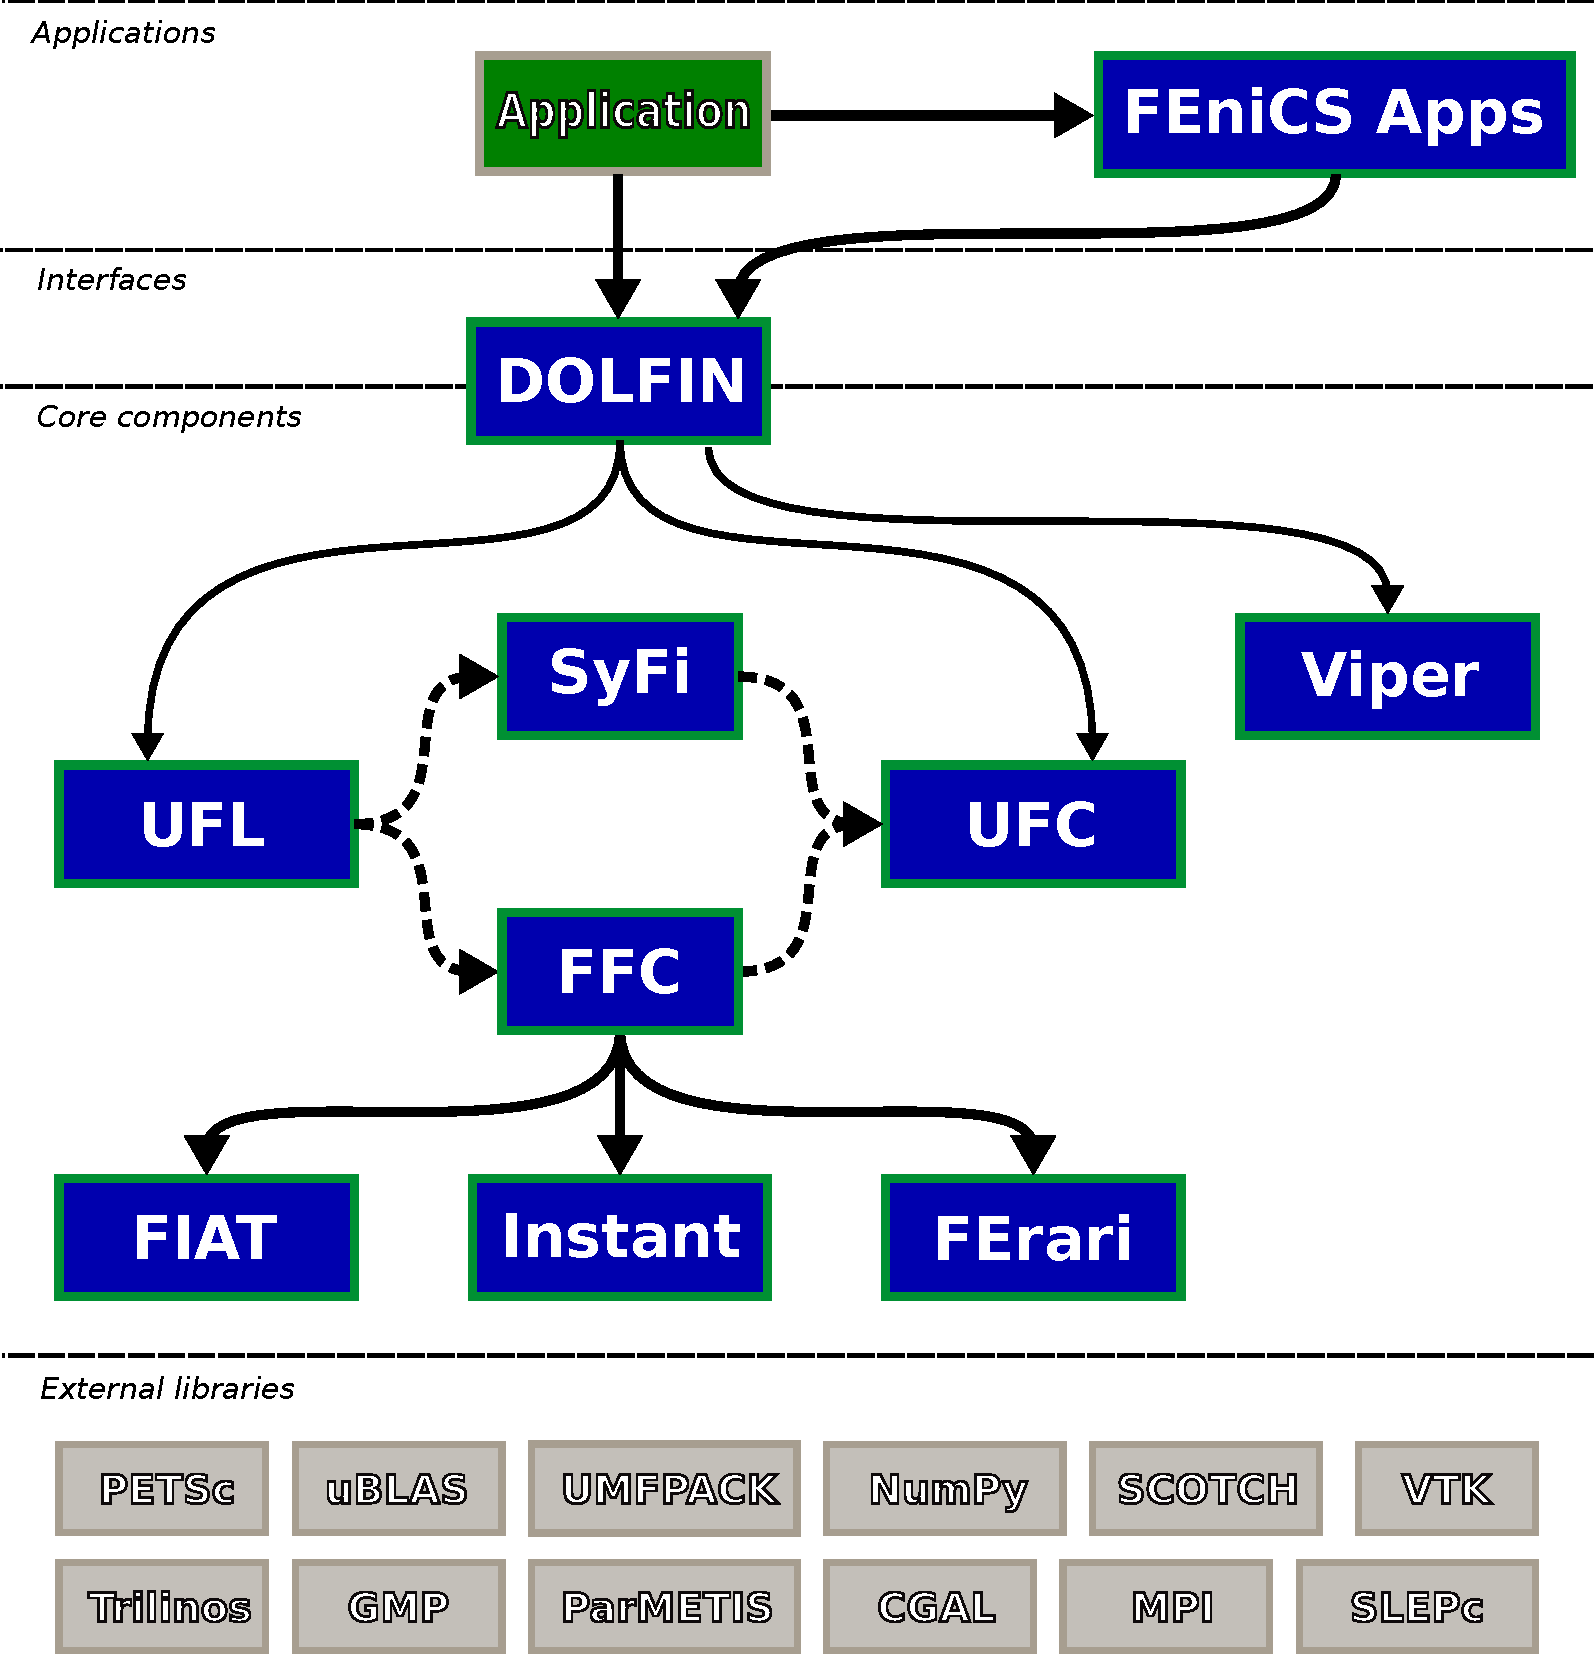
\includegraphics[width=\largefig]{chapters/logg-2/pdf/fenics-map.pdf}
  \caption{DOLFIN functions as the main user interface of FEniCS and
    handles the communication between the various components of FEniCS
    and external software. Solid lines indicate dependencies and
    dashed lines indicate data flow.}
  \label{fig:logg-2:fenicsmap}
\end{figure}

%------------------------------------------------------------------------------
%------------------------------------------------------------------------------
\section{User interfaces}

DOLFIN provides two user interfaces. One interface is implemented as a
traditional C++ library, and another interface is implemented as a
standard Python module. The two interfaces are near-identical, but in
some cases particular language features of either C++ or Python
require variations in the interfaces.  In particular, the Python
interface adds an additional level of automation by employing
run-time (just-in-time) code generation.  Below, we comment on the
design and implementation of the two user interfaces of DOLFIN.

%------------------------------------------------------------------------------
\subsection{C++ interface}

The DOLFIN C++ interface is designed as a standard object-oriented
C++ library. It provides classes such as \emp{Matrix}, \emp{Vector},
\emp{Mesh}, \emp{FiniteElement}, \emp{FunctionSpace} and \emp{Function},
which model important concepts for finite element computing (see
Figure~\ref{fig:logg-2:uml}). It also provides a small number of free
functions (a function that is not a member function of a class),
most notably \emp{assemble} and \emp{solve}, which can be used in
conjunction with DOLFIN class objects to implement finite element
solvers. The interface is designed to be as simple as possible, and
without compromising on generality.  When external software is wrapped,
a simple and consistent user interface is provided to allow the rapid
development of solvers without needing to deal with differences in the
interfaces of external libraries. However, DOLFIN has been designed to
interact flexibly with external software. In particular, in cases where
DOLFIN provides wrappers for external libraries, such as the \emp{Matrix}
and \emp{Vector} classes which wrap data structures from linear algebra
libraries like PETSc and Trilinos, advanced users may, if necessary,
access the underlying data structures in order to use native functionality
from the wrapped external libraries.

\begin{figure}
  \begin{center}
    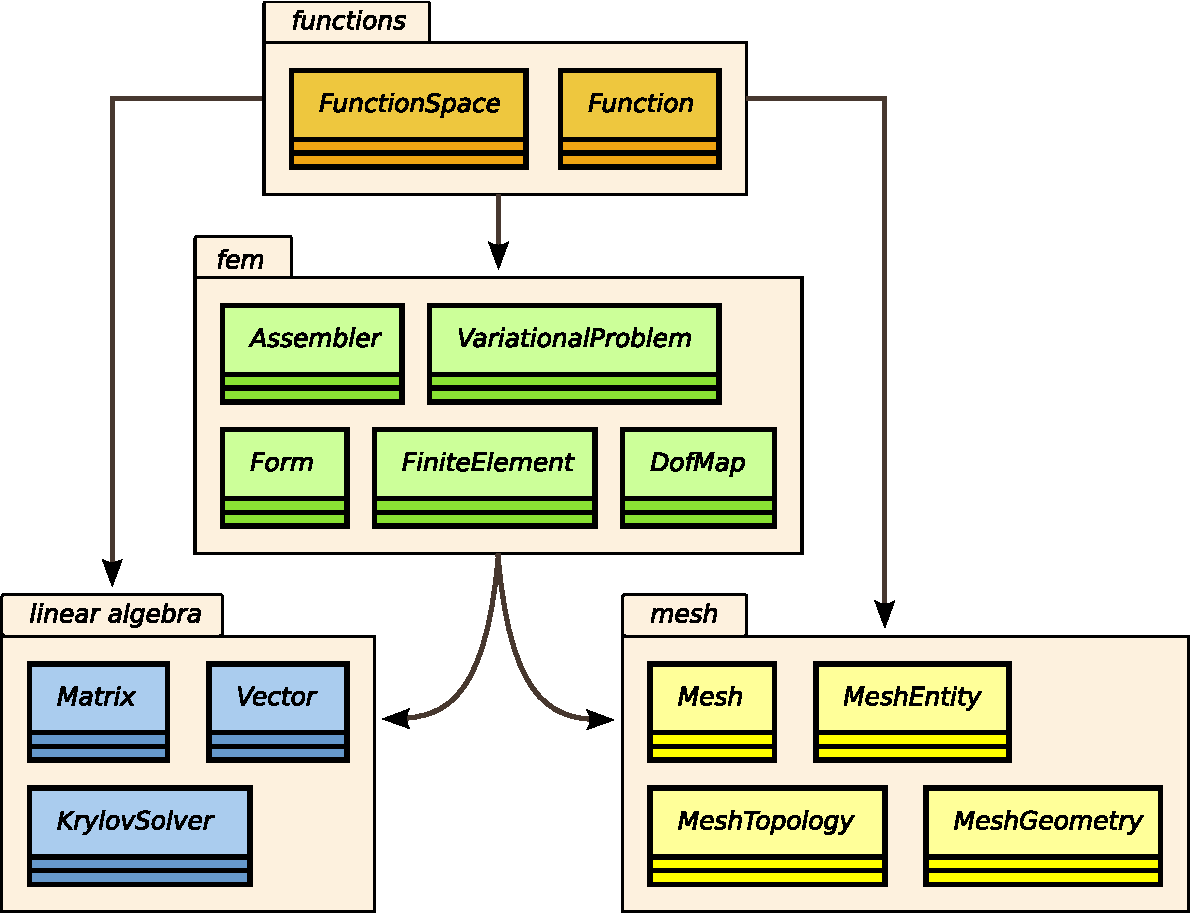
\includegraphics[width=\largefig]{chapters/logg-2/pdf/dolfin-uml.pdf}
    \caption{Schematic overview of some of the most important components
    and classes of DOLFIN. Arrows indicate dependencies.}
    \label{fig:logg-2:uml}
  \end{center}
\end{figure}

To solve partial differential equations using the DOLFIN C++
interface, users must express finite element variational problems
in the UFL form language. This is accomplished by entering the forms
into separate \emp{.ufl} files and compiling those files using a form
compiler to generate UFC-compliant C++ code. The generated code may
then be included in a DOLFIN C++ program. We return to this issue in
Section~\ref{sec:logg-2:functionality}.

To use DOLFIN from C++, users need to include one or more header files
from the DOLFIN C++ library. In the simplest case, one includes the
header file \emp{dolfin.h}, which in turn includes all other DOLFIN
header files:

\begin{c++}
#include <dolfin.h>

using namespace dolfin;

int main()
{

  return 0;
}
\end{c++}

%------------------------------------------------------------------------------
\subsection{Python interface}

Over the last decade, Python has emerged as an attractive choice for
the rapid development of simulation codes for scientific computing.
Python brings the benefits of a high-level scripting language, the
strength of an object-oriented language and a wealth of libraries for
numerical computation.

The bulk of the DOLFIN Python interface is automatically generated from
the C++ interface using SWIG. As a consequence, users may implement
DOLFIN-based solvers that appear very similar in C++ and Python. Since
the functionality of both the C++ and Python interfaces are implemented
as part of the DOLFIN C++ library, DOLFIN is equally efficient via the
C++ and Python interfaces for most operations.

Python offers possibilities that are not available in C++. The Python
interface can therefore provide some functionality that is not available
from the C++ interface. In particular, the UFL form language is seamlessly
integrated into the Python interface and code generation is automatically
handled at run-time.  To use DOLFIN from Python, users need to import
functionality from the DOLFIN Python module. In the simplest case,
one includes all functionality from the Python module named \emp{dolfin}:

\begin{python}
from dolfin import *
\end{python}

%------------------------------------------------------------------------------
%------------------------------------------------------------------------------
\section{Functionality}
\label{sec:logg-2:functionality}

DOLFIN is organized as a collection of libraries (modules), with each
covering a certain area of functionality. We review here these areas
and explain the purpose and usage of the most commonly used classes and
functions. The review is bottom-up; that is, we start by describing the
core low-level functionality of DOLFIN (linear algebra and meshes) and
then move upwards to describe higher level functionality. For further
details, we refer to the FEniCS Programmer's Reference on the FEniCS
Project web page and to \citet{LoggWells2010}.

%------------------------------------------------------------------------------
\subsection{Linear algebra}

DOLFIN provides a range of linear algebra objects and functionality,
including vectors, dense and sparse matrices, direct and iterative linear
solvers and eigenvalues solvers, and does so via a simple and consistent
interface.  For the bulk of underlying functionality, DOLFIN relies
on third-party libraries such as PETSc and Trilinos.  DOLFIN defines
the abstract base classes \emp{GenericTensor}, \emp{GenericMatrix}
and \emp{GenericVector}, and these are used extensively throughout the
library.  Implementations of these generic interfaces for a number of
backends are provided in DOLFIN, thereby achieving a common interface for
different backends.  Users can also wrap other linear algebra backends
by implementing the generic interfaces.

\paragraph{Matrices and vectors.}

The simplest way to create matrices and vectors is via the classes
\emp{Matrix} and \emp{Vector}. In general, \emp{Matrix} and \emp{Vector}
represent distributed linear algebra objects that may be stored across
(MPI) processes when running in parallel. Consistent with the most common
usage in a finite element library, a \emp{Vector} uses dense storage
and a \emp{Matrix} uses sparse storage.  A \emp{Vector} can be created
as follows:

\begin{c++}
Vector x;
\end{c++}

\begin{python}
x = Vector()
\end{python}
and a matrix can be created by:

\begin{c++}
Matrix A;
\end{c++}

\begin{python}
A = Matrix()
\end{python}
In most applications, a user may need to create a matrix or a vector,
but most operations on the linear algebra objects, including resizing,
will take place inside the library and a user will not have to operate
on the objects directly.

The following code illustrates how to create a vector of size~100:
%%
\begin{c++}
Vector x(100);
\end{c++}
%%
\begin{python}
x = Vector(100)
\end{python}
%%
A number of backends support distributed linear algebra for parallel
computation, in which case the vector \emp{x} will have global size
100, and DOLFIN will partition the vector across processes in (near)
equal-sized portions.

%To control the distribution of a vector across processes, for example,
%to match to the dimensions of locally owned degrees of freedom, a
%\emp{Vector} can be created using a local (process) range. For
%example, a vector that stores entries 20 to 79 on the local process is
%created by:
%
%\begin{c++}
%Vector x(20, 80);
%\end{c++}
%
%\begin{python}
%x = Vector(20, 80)
%\end{python}
%The vector must be created on all processes and there must be no overlap
%in the local ranges. The linear algebra backend will compute the global
%size of the vector based on the local size for each process.

Creating a \emp{Matrix} of a given size is more involved as the matrix
is sparse and in general needs to be initialized (data structures
allocated) based on the structure of the sparse matrix (its sparsity
pattern). Initialization of sparse matrices is handled by DOLFIN when
required.

While DOLFIN supports distributed linear algebra objects for parallel
computation, it is rare that a user is exposed to details at the level
of parallel data layouts. The distribution of objects across processes
is handled automatically by the library.

\paragraph{Solving linear systems.}

The simplest approach to solving the linear system $Ax = b$ is to use
%
\begin{c++}
solve(A, x, b);
\end{c++}
%
\begin{python}
solve(A, x, b)
\end{python}
%
DOLFIN will use a default method to solve the system of equations.
Using the function \emp{solve} is straightforward, but it offers little
control over details of the solution process. For many applications, it is
desirable to exercise a degree of control over the solution process.
It is possible in DOLFIN to select the solver type (direct or iterative)
and to control details of the solution method, and this is expanded upon
below.

The linear system $Ax = b$ can be solved using LU decomposition
(a direct method) as follows:
%
\begin{c++}
LUSolver solver(A);
solver.solve(x, b);
\end{c++}
%
\begin{python}
solver = LUSolver(A)
solver.solve(x, b)
\end{python}
%
Alternatively, the operator $A$ associated with the linear solver
can be set post-construction:
%
\begin{c++}
LUSolver solver;
solver.set_operator(A);
solver.solve(x, b);
\end{c++}
%
\begin{c++}
solver = LUSolver()
solver.set_operator(A)
solver.solve(x, b)
\end{c++}
%
This can be useful when passing a linear solver via a function
interface and setting the operator inside a function.

In some cases, the system $Ax = b$ may be solved a number of times for
a given $A$, or for different $A$ but with the same non-zero structure.
If the nonzero structure of $A$ does not change, then some efficiency
gains for repeated solves can be achieved by informing the LU solver:

\begin{c++}
solver.parameters["same_nonzero_pattern"] = true;
\end{c++}

\begin{python}
solver.parameters["same_nonzero_pattern"] = True
\end{python}
In the case that $A$ does not change, the solution time for subsequent
solves can be reduced dramatically by re-using the LU factorization
of~$A$.  Re-use of the factorization is controlled by the parameter
\emp{"reuse\_factorization"}.

It is possible for some backends to prescribe the specific LU solver
to be used. This depends on the backend, which solvers have been
configured by DOLFIN and how third-party linear algebra backends have
been configured.

The system of equations $Ax = b$ can be solved using a preconditioned
Krylov solver by:

\begin{c++}
KrylovSolver solver(A);
solver.solve(x, b);
\end{c++}

\begin{python}
solver = KrylovSolver(A)
solver.solve(x, b)
\end{python}
The above will use a default preconditioner and solver, and default
parameters. If a \emp{KrylovSolver} is constructed without a matrix
operator $A$, the operator can be set post-construction:

\begin{c++}
KrylovSolver solver;
solver.set_operator(A);
\end{c++}

\begin{python}
solver = KrylovSolver()
solver.set_operator(A)
\end{python}
In some cases, it may be useful to use a preconditioner matrix $P$ that
differs from~$A$:

\begin{c++}
KrylovSolver solver;
solver.set_operators(A, P)
\end{c++}

\begin{python}
solver = KrylovSolver()
solver.set_operators(A, P)
\end{python}
Various parameters for Krylov solvers can be set. Some common parameters
are:

\begin{python}
solver = KrylovSolver()
solver.parameters["relative_tolerance"]      = 1.0e-6
solver.parameters["absolute_tolerance"]      = 1.0e-15
solver.parameters["divergence_limit"]        = 1.0e4
solver.parameters["maximum_iterations"]      = 1.0e4
solver.parameters["error_on_nonconvergence"] = True
solver.parameters["nonzero_initial_guess"]   = False
\end{python}
The parameters may be set similarly from C++. Printing a summary of
the convergence of a \emp{KrylovSolver} and printing details of the
convergence history can be controlled via parameters:

\begin{c++}
KrylovSolver solver;
solver.parameters["report"] = true;
solver.parameters["monitor_convergence"] = true;
\end{c++}

\begin{python}
solver = KrylovSolver()
solver.parameters["report"] = True
solver.parameters["monitor_convergence"] = True
\end{python}
The specific Krylov solver and preconditioner to be used can be set at
construction of a solver object. The simplest approach is to set the
Krylov method and the preconditioner via string descriptions. For example:

\begin{c++}
KrylovSolver solver("gmres", "ilu");
\end{c++}

\begin{python}
solver = KrylovSolver("gmres", "ilu")
\end{python}
The above specifies the Generalized Minimum Residual (GMRES) method as
a solver, and incomplete LU (ILU) preconditioning. The available
methods and preconditioners depend on the configured backends, but
common methods, such as GMRES (\emp{"gmres"}), the Conjugate Gradient method
(\emp{"cg"}) and ILU preconditioning (\emp{"ilu"}) are available for all backends.

When backends such as PETSc and Trilinos are configured, a wide range
of Krylov methods and preconditioners can be applied, and a large number
of solver and preconditioner parameters can be set. In addition to what
is described here, DOLFIN provides more advanced interfaces which permit
finer control of the solution process. It is also possible for users to
provide their own preconditioners.

\paragraph{Solving eigenvalue problems.}

DOLFIN uses the library SLEPc, which builds on PETSc, to solve eigenvalue
problems. The SLEPc interface works only with PETSc-based linear algebra
objects.  Therefore it is necessary to use PETSc-based objects, or to
set the default linear algebra backend to PETSc and downcast objects
(as explained in the next section). The following code illustrates
the solution of the eigenvalue problem $Ax = \lambda x$:
%%
\begin{c++}
// Create matrix
PETScMatrix A;

// Code omitted for setting the entries of A

// Create eigensolver
SLEPcEigenSolver eigensolver(A);

// Compute all eigenvalues of A
eigensolver.solve();

// Get first eigenpair
double lambda_real, lambda_complex;
PETScVector x_real, x_complex;
eigensolver.get_eigenpair(lambda_real, lambda_complex, x_real, x_complex, 0);
\end{c++}
%%
\begin{python}
# Create matrix
A = PETScMatrix()

# Code omitted for setting the entries of A

# Create eigensolver
eigensolver = SLEPcEigenSolver(A)

# Compute all eigenvalues of A
eigensolver.solve()

# Get first eigenpair
lambda_r, lambda_c, x_real, x_complex = eigensolver.get_eigenpair(0)
\end{python}
%%
The real and complex components of the eigenvalue are returned in
\emp{lambda\_real} and \emp{lambda\_complex}, respectively, and the
real and complex components of the eigenvector are
returned in \emp{x\_real} and \emp{x\_complex}, respectively.

To create a solver for the generalized eigenvalue problem $Ax = \lambda Mx$, the
eigensolver can be constructed using $A$ and~$M$:

\begin{c++}
PETScMatrix A;
PETScMatrix M;

// Code omitted for setting the entries of A and M

SLEPcEigenSolver eigensolver(A, M);
\end{c++}
\begin{python}
A = PETScMatrix()
M = PETScMatrix()

# Code omitted for setting the entries of A and M

eigensolver = SLEPcEigenSolver(A, M)
\end{python}
There are a wide number of options that a user can set via the
parameter system to control the eigenproblem solution process. To
print a list of available parameters, call
\emp{info(eigensolver.parameters, true)} and
\emp{info(eigensolver.parameters, True)} from C++ and Python,
respectively.

\paragraph{Selecting a linear algebra backend.}

The \emp{Matrix}, \emp{Vector}, \emp{LUSolver} and \emp{KrylovSolver}
objects are all based on a specific linear algebra backend.
The default backend depends on which backends are enabled when DOLFIN
is configured.  The linear algebra backend can be set via the global
parameter \emp{"linear\_algebra\_backend"}.  To use PETSc as the linear
algebra backend:
%%
\begin{c++}
parameters["linear_algebra_backend"] = "PETSc";
\end{c++}
%%
\begin{python}
parameters["linear_algebra_backend"] = "PETSc"
\end{python}
%%
This parameter should be set before creating linear algebra
objects. To use Epetra from the Trilinos collection, the parameter
\emp{"linear\_algebra\_backend"} should be set to \emp{"Epetra"}.
For uBLAS, the parameter should be set to \emp{"uBLAS"} and for MTL4, the
parameter should be set to \emp{"MTL4"}.

Users can explicitly create linear algebra objects that use a
particular backend. Generally, such objects are prefixed with the name
of the backend. For example, a PETSc-based vector and LU solver are
created by:
%%
\begin{c++}
PETScVector x;
PETScLUSolver solver;
\end{c++}
%%
\begin{python}
x = PETScVector()
solver = PETScLUSolver()
\end{python}


\paragraph{Solving nonlinear systems.}

DOLFIN provides a Newton solver in the form of the class
\emp{NewtonSolver} for solving nonlinear systems of equations of the
form
%%
\begin{equation}
  F(x) = 0,
\end{equation}
%%
where $x \in \mathbb{R}^{n}$ and $F: \mathbb{R}^{n} \rightarrow
\mathbb{R}^{n}$. To solve such a problem using the DOLFIN Newton
solver, a user needs to provide a subclass of \emp{NonlinearProblem}.
The purpose of a \emp{NonlinearProblem} object is to evaluate $F$ and
the Jacobian of $F$, which will be denoted by~$J: \mathbb{R}^{n}
\rightarrow \mathbb{R}^{n} \times \mathbb{R}^{n}$. An outline of a
user-provided \emp{MyNonlinearProblem} class for solving a nonlinear
differential equation is shown below.
%%
\begin{c++}
class MyNonlinearProblem : public NonlinearProblem
{
public:

  // Constructor
  MyNonlinearProblem(const Form& L, const Form& a,
                     const BoundaryCondition& bc) : L(L), a(a), bc(bc) {}

  // User-defined residual vector F
  void F(GenericVector& b, const GenericVector& x)
  {
    assemble(b, L);
    bc.apply(b, x);
  }

  // User-defined Jacobian matrix J
  void J(GenericMatrix& A, const GenericVector& x)
  {
    assemble(A, a);
    bc.apply(A);
  }

private:

  const Form& L;
  const Form& a;
  const BoundaryCondition& bc;

};
\end{c++}
%%
A \emp{MyNonlinearProblem} object is constructed using a linear form
\emp{L}, that when assembled corresponds to $F$, and a bilinear form
\emp{a}, that when assembled corresponds to~$J$. The classes \emp{Form}
and \emp{BoundaryCondition} used in the example are discussed in more
detail later.  The same \emp{MyNonlinearProblem} class can be defined
in Python:
%%
\begin{python}
class MyNonlinearProblem(NonlinearProblem):
    def __init__(self, L, a, bc):
        NonlinearProblem.__init__(self)
        self.L = L
        self.a = a
        self.bc = bc
    def F(self, b, x):
        assemble(self.L, tensor=b)
        self.bc.apply(b, x)
    def J(self, A, x):
        assemble(self.a, tensor=A)
        self.bc.apply(A)
\end{python}

Once a nonlinear problem class has been defined, a \emp{NewtonSolver}
object can be created and the Newton solver can be used to compute
the solution vector $x$ to the nonlinear problem:
%%
\begin{c++}
MyNonlinearProblem problem(L, a, bc);
NewtonSolver newton_solver;

Vector x;
newton_solver.solve(problem, x);
\end{c++}
%%
\begin{python}
problem = MyNonlinearProblem(L, a, bc)
newton_solver = NewtonSolver()

x = Vector()
newton_solver.solve(problem, x)
\end{python}
%%
A number of parameters can be set for a \emp{NewtonSolver}. Some
parameters that determine the behavior of the Newton solver are:
%%
\begin{python}
newton_solver = NewtonSolver()
newton_solver.parameter["maximum_iterations"] = 20
newton_solver.parameter["relative_tolerance"] = 1.0e-6
newton_solver.parameter["absolute_tolerance"] = 1.0e-10
newton_solver.parameter["error_on_nonconvergence"] = False
\end{python}
%%
The parameters may be set similarly from~C++.  When testing for
convergence, usually a norm of the residual $F$ is checked.  Sometimes it
is useful instead to check a norm of the the iterative correction~$dx$.
This is controlled by the parameter \emp{"convergence\_criterion"}, which
can be set to \emp{"residual"}, for checking the size of the residual $F$,
or \emp{"incremental"}, for checking the size of the increment~$dx$.

For more advanced usage, a \emp{NewtonSolver} can be constructed with
arguments that specify the linear solver and preconditioner to be used
in the solution process.

%------------------------------------------------------------------------------
\subsection{Meshes}

A central part of DOLFIN is its mesh library and the \emp{Mesh}
class. The mesh library provides data structures and algorithms for
computational meshes, including the computation of mesh connectivity
(incidence relations), mesh refinement, mesh partitioning and mesh
intersection.

The mesh library is implemented in C++ and has been optimized to
minimize storage requirements and to enable efficient access to mesh
data. In particular, a DOLFIN mesh is stored in a small number of
contiguous arrays, on top of which a light-weight object-oriented
layer provides a~\emph{view} to the underlying data. For a detailed
discussion on the design and implementation of the mesh library, we
refer to \citet{Logg2009}.

\paragraph{Creating a mesh.}

DOLFIN provides functionality for creating simple meshes, such as
meshes of unit squares and unit cubes, spheres, rectangles and
boxes. The following code demonstrates how to create a $16\times 16$
triangular mesh of the unit square (consisting of $2\times 16\times 16
= 512$ triangles) and a $16\times 16\times 16$ tetrahedral mesh of the
unit cube (consisting of $6\times 16\times 16\times 16 = 24,576$
tetrahedra).

\begin{c++}
UnitSquare unit_square(16, 16);
UnitCube unit_cube(16, 16, 16);
\end{c++}

\begin{python}
unit_square = UnitSquare(16, 16)
unit_cube = UnitCube(16, 16, 16)
\end{python}

Simplicial meshes (meshes consisting of intervals, triangles or
tetrahedra) may be constructed explicitly by specifying the cells and
vertices of the mesh. An interface for creating simplicial meshes is
provided by the class \texttt{MeshEditor}. The following code
demonstrates how to create a mesh consisting of two triangles covering
the unit square.

\begin{c++}
Mesh mesh;
MeshEditor editor;
editor.open(mesh, 2, 2);
editor.init_vertices(4);
editor.init_cells(2);
editor.add_vertex(0, 0.0, 0.0);
editor.add_vertex(1, 1.0, 0.0);
editor.add_vertex(2, 1.0, 1.0);
editor.add_vertex(3, 0.0, 1.0);
editor.add_cell(0, 0, 1, 2);
editor.add_cell(1, 0, 2, 3);
editor.close();
\end{c++}

\begin{python}
mesh = Mesh();
editor = MeshEditor();
editor.open(mesh, 2, 2)
editor.init_vertices(4)
editor.init_cells(2)
editor.add_vertex(0, 0.0, 0.0)
editor.add_vertex(1, 1.0, 0.0)
editor.add_vertex(2, 1.0, 1.0)
editor.add_vertex(3, 0.0, 1.0)
editor.add_cell(0, 0, 1, 2)
editor.add_cell(1, 0, 2, 3)
editor.close()
\end{python}

\paragraph{Reading a mesh from file.}

Although the built-in classes \emp{UnitSquare} and \emp{UnitCube}
are useful for testing, a typical application will need to read from
file a mesh that has been generated by an external mesh generator. To read
a mesh from file, simply supply the filename to the constructor of the
\emp{Mesh} class:
%%
\begin{c++}
Mesh mesh("mesh.xml");
\end{c++}
%%
\begin{python}
mesh = Mesh("mesh.xml")
\end{python}
%%
Meshes must be stored in the DOLFIN XML format. The following example
illustrates how to store a $2 \times 2$ mesh of the unit square:

\begin{xml}
<?xml version="1.0" encoding="UTF-8"?>

<dolfin xmlns:dolfin="http://www.fenicsproject.org">
  <mesh celltype="triangle" dim="2">
    <vertices size="9">
      <vertex index="0" x="0" y="0"/>
      <vertex index="1" x="0.5" y="0"/>
      <vertex index="2" x="1" y="0"/>
      <vertex index="3" x="0" y="0.5"/>
      <vertex index="4" x="0.5" y="0.5"/>
      <vertex index="5" x="1" y="0.5"/>
      <vertex index="6" x="0" y="1"/>
      <vertex index="7" x="0.5" y="1"/>
      <vertex index="8" x="1" y="1"/>
    </vertices>
    <cells size="8">
      <triangle index="0" v0="0" v1="1" v2="4"/>
      <triangle index="1" v0="0" v1="3" v2="4"/>
      <triangle index="2" v0="1" v1="2" v2="5"/>
      <triangle index="3" v0="1" v1="4" v2="5"/>
      <triangle index="4" v0="3" v1="4" v2="7"/>
      <triangle index="5" v0="3" v1="6" v2="7"/>
      <triangle index="6" v0="4" v1="5" v2="8"/>
      <triangle index="7" v0="4" v1="7" v2="8"/>
    </cells>
  </mesh>
</dolfin>
\end{xml}
%%
Meshes stored in other data formats may be converted to the DOLFIN XML
format using the command \emp{dolfin-convert}, as explained in more
detail below.

\paragraph{Mesh entities.}

Conceptually, a \emph{mesh} (modeled by the class \emp{Mesh}), consists of
a collection of \emph{mesh entities}.  A \emph{mesh entity} is a pair $(d,
i)$, where $d$ is the topological dimension of the mesh entity and $i$
is a unique index of the mesh entity. Mesh entities are numbered within
each topological dimension from $0$ to $n_d-1$, where $n_d$ is the number
of mesh entities of topological dimension~$d$.

\begin{figure}
  \begin{center}
    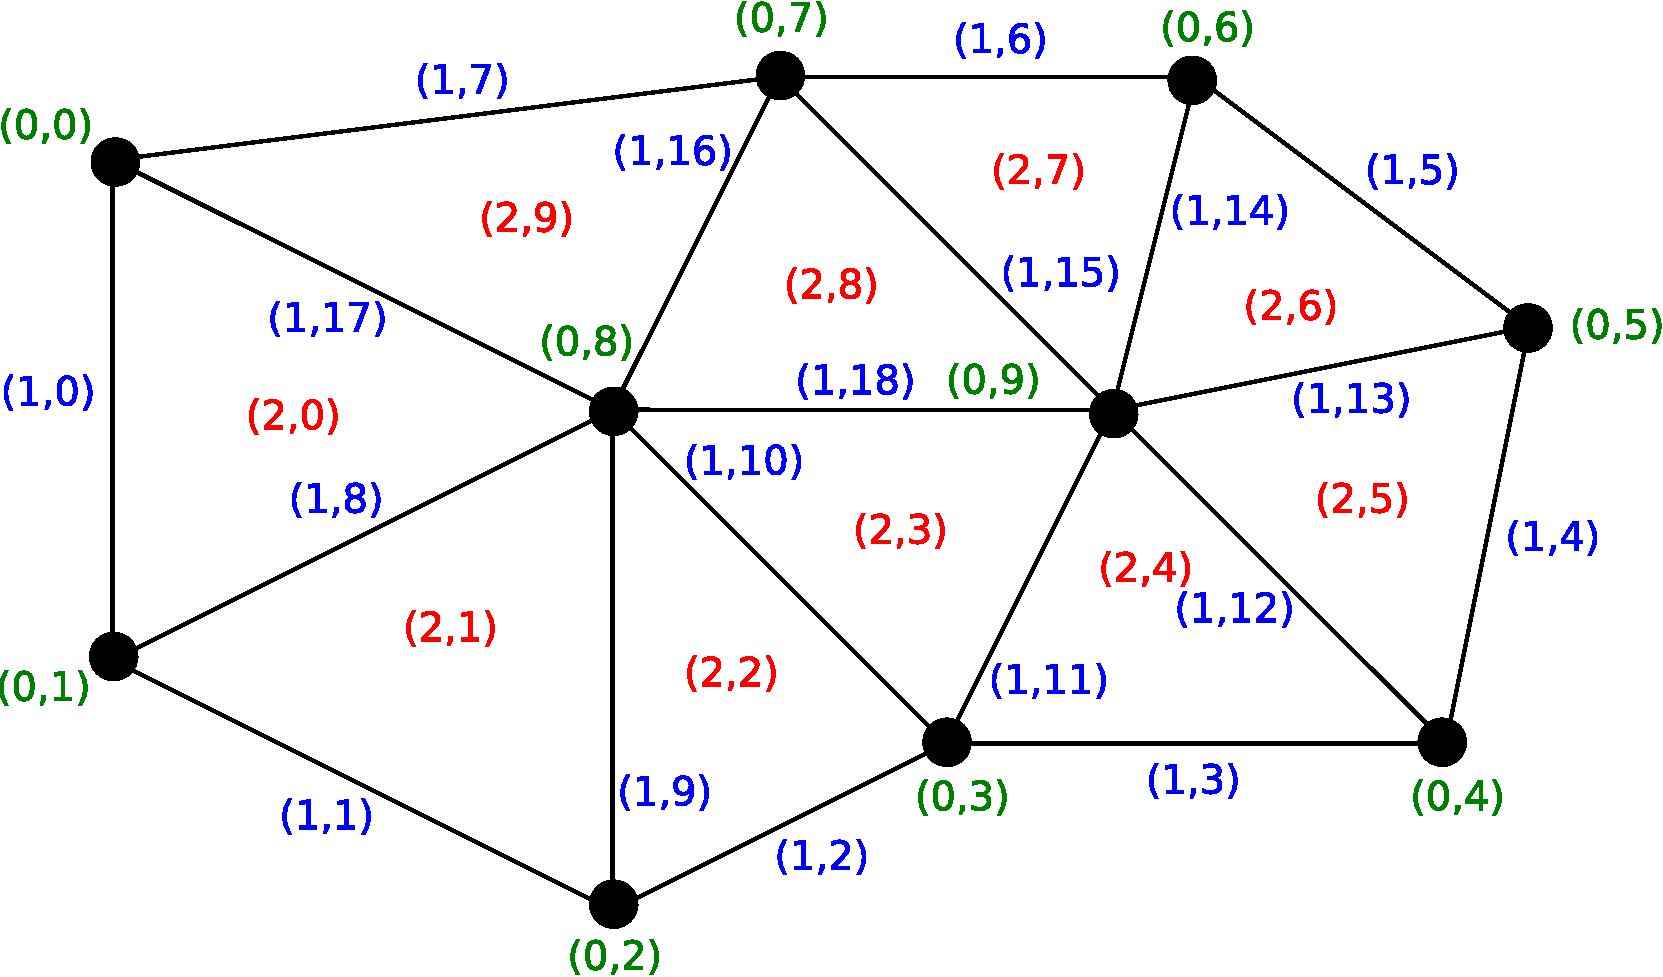
\includegraphics[width=\largefig]{chapters/logg-2/pdf/mesh-p1-entities.pdf}
    \caption{Each entity of a mesh is identified by a pair $(d, i)$
      which specifies the topological dimension~$d$ and a unique
      index~$i$ for the entity within the set of entities of
      dimension~$d$.}
    \label{fig:logg-2:entities}
  \end{center}
\end{figure}

For convenience, mesh entities of topological dimension~$0$ are
referred to as \emph{vertices}, entities of dimension~$1$ as
\emph{edges}, entities of dimension~$2$ as \emph{faces}. Entities of
\emph{codimension}~$1$ are referred to as \emph{facets} and entities
of codimension~$0$ as \emph{cells}. These concepts are summarized in
Figure~\ref{fig:logg-2:entities} and
Table~\ref{tab:logg-2:entities}. We note that a triangular mesh
consists of vertices, edges and cells, and that the edges may
alternatively be referred to as facets and the cells as faces. We
further note that a tetrahedral mesh consists of vertices, edges,
faces and cells, and that the faces may alternatively be referred to
as facets. These concepts are implemented by the classes
\texttt{MeshEntity}, \texttt{Vertex}, \texttt{Edge}, \texttt{Face},
\texttt{Facet} and \texttt{Cell}. These classes do not store any
data. Instead, they are light-weight objects that provide views of the
underlying mesh data. A \emp{MeshEntity} may be created from a
\emp{Mesh}, a topological dimension and an index. The following code
demonstrates how to create various entities on a mesh.
%%
\begin{c++}
MeshEntity entity(mesh, 0, 33); // vertex number 33
Vertex vertex(mesh, 33);        // vertex number 33
Cell cell(mesh, 25);            // cell number 25
\end{c++}
%%
\begin{python}
entity = MeshEntity(mesh, 0, 33) # vertex number 33
vertex = Vertex(mesh, 33)        # vertex number 33
cell = Cell(mesh, 25)            # cell number 25
\end{python}

\begin{table}
  \begin{center}
    \begin{tabular}{lcc}
      \toprule
      Entity & Dimension & Codimension \\
      \hline
      Vertex & $0$ & $D$ \\
      Edge & $1$ & $D-1$ \\
      Face & $2$ & $D-2$ \\
      & & \\
      Facet & $D-1$ & $1$ \\
      Cell & $D$ & $0$ \\
      \bottomrule
    \end{tabular}
    \caption{Mesh entities and their dimensions/codimensions. The
      codimension of an entity is $D - d$ where $D$ is the maximal
      dimension and $d$ is the dimension.}
  \end{center}
  \label{tab:logg-2:entities}
\end{table}

\paragraph{Mesh topology and geometry.}

The topology of a mesh is stored separately from its geometry. The
topology of a mesh is a description of the relations between the
various entities of the mesh, while the geometry describes how those
entities are embedded in $\R^d$.

Users are rarely confronted with the \emp{MeshTopology} and
\emp{MeshGeometry} classes directly since most algorithms on meshes can be
expressed in terms of \emph{mesh iterators}. However, users may sometimes
need to access the dimension of a \emp{Mesh}, which involves accessing
either the \emp{MeshTopology} or \emp{MeshGeometry}, which are stored
as part of the \emp{Mesh}, as illustrated in the following code examples:
%%
\begin{c++}
uint gdim = mesh.topology().dim();
uint tdim = mesh.geometry().dim();
\end{c++}
%%
\begin{python}
gdim = mesh.topology().dim()
tdim = mesh.geometry().dim()
\end{python}
%%
It should be noted that the topological and geometric dimensions may
differ. This is the case in particular for the boundary of a mesh,
which is typically a mesh of topological dimension~$D$ embedded in
$\R^{D+1}$. That is, the geometry dimension is~$D + 1$.

\paragraph{Mesh connectivity.}

The topology of a \emp{Mesh} is represented by the \emph{connectivity}
(incidence relations) of the mesh, which is a complete description of
which entities of the mesh are connected to which entities. Such
connectivity is stored in DOLFIN by the \emp{MeshConnectivity}
class. One such data set is stored as part of the class
\emp{MeshTopology} for each pair of topological dimensions $d
\rightarrow d'$ for $d, d' = 0, 1, \ldots, D$, where $D$ is the
topological dimension.

When a \emp{Mesh} is created, a minimal \emp{MeshTopology} is created.
Only the connectivity from cells (dimension~$D$) to vertices
(dimension~$0$) is stored (\emp{MeshConnectivity} $D \rightarrow 0$).
When a certain connectivity is requested, such as for example the connectivity
$1 \rightarrow 1$ (connectivity from edges to edges), DOLFIN automatically
computes any other connectivities required for computing the requested
connectivity. This is illustrated in Table~\ref{tab:logg-2:connectivity},
where we indicate which connectivities are required to compute the $1
\rightarrow 1$ connectivity.  The following code demonstrates how to
initialize various kinds of mesh connectivity for a tetrahedral mesh
($D = 3$).
%%
\begin{c++}
mesh.init(2);    // Compute faces
mesh.init(0, 0); // Compute vertex neighbors for each vertex
mesh.init(1, 1); // Compute edge neighbors for each edge
\end{c++}
%%
\begin{python}
mesh.init(2)      # Compute faces
mesh.init(0, 0)   # Compute vertex neighbors for each vertex
mesh.init(1, 1)   # Compute edge neighbors for each edge
\end{python}

\begin{table}
  \begin{center}
    \begin{tabular}{c|cccc}
      & 0 & 1 & 2 & 3 \\
      \hline
      0 & -- & $\times$ & -- & $\times$ \\
      1 & $\times$ & $\times$ & -- & -- \\
      2 & -- & -- & -- & -- \\
      3 & $\times$ & $\times$ & -- & $\times$ \\
    \end{tabular}
  \end{center}
  \caption{DOLFIN computes the connectivity $d \rightarrow d'$ of a
    mesh for any pair $d, d' = 0, 1, \ldots, D$. The table
    indicates which connectivity pairs (indicated by~$\times$) have
    been computed in order to compute the connectivity $1 \rightarrow
    1$ (edge--edge connectivity) for a tetrahedral mesh.}
\label{tab:logg-2:connectivity}
\end{table}

\paragraph{Mesh iterators.}

Algorithms operating on a mesh can often be expressed in terms of
\emph{iterators}. The mesh library provides the general iterator
\texttt{MeshEntityIterator} for iteration over mesh entities,
as well as the specialized mesh iterators \texttt{VertexIterator},
\texttt{EdgeIterator}, \texttt{FaceIterator}, \texttt{FacetIterator}
and \texttt{Cell\-Iterator}.

The following code illustrates how to iterate over all incident
(connected) vertices of all vertex neighbors of all cells of a given
mesh. The code implies that two vertices are considered as neighbors if
they both belong to the same cell. For simplex meshes, this is equivalent
to an edge connecting the two vertices.
%%
\begin{c++}
for (CellIterator c(mesh); !c.end(); ++c)
  for (VertexIterator v0(*c); !v0.end(); ++v0)
    for (VertexIterator v1(*v0); !v1.end(); ++v1)
      cout << *v1 << endl;
\end{c++}
%%
\begin{python}
for c in cells(mesh):
    for v0 in vertices(c):
        for v1 in vertices(v0):
            print v1
\end{python}
%%
This may alternatively be implemented using the general iterator
\emp{MeshEntity\-Iterator} as follows:
%%
\begin{c++}
uint D = mesh.topology().dim();
for (MeshEntityIterator c(mesh, D); !c.end(); ++c)
  for (MeshEntityIterator v0(*c, 0); !v0.end(); ++v0)
    for (MeshEntityIterator v1(*v0, 0); !v1.end(); ++v1)
      cout << *v1 << endl;
\end{c++}
%%
\begin{python}
D = mesh.topology().dim()
for c in entities(mesh, D):
    for v0 in entities(c, 0):
        for v1 in entities(v0, 0):
            print v1
\end{python}

\paragraph{Mesh functions.}

A useful class for storing data associated with a \emp{Mesh} is the
\emp{MeshFunction} class. This makes it simple to store, for example,
material parameters, subdomain indicators, refinement markers on the
\emp{Cell}s of a \emp{Mesh} or boundary markers on the \emp{Facet}s of
a \emp{Mesh}.  A \texttt{MeshFunction} is a discrete function that takes
a value on each mesh entity of a given topological dimension~$d$. The
number of values stored in a \emp{MeshFunction} is equal to the number
of entities $n_d$ of dimension~$d$. A \texttt{MeshFunction} is templated
over the value type and may thus be used to store values of any
type. For convenience, named \texttt{MeshFunction}s are provided by the
classes \emp{VertexFunction}, \emp{EdgeFunction}, \emp{FaceFunction},
\emp{FacetFunction} and \emp{CellFunction}.  The following code
illustrates how to create a pair of \emp{MeshFunction}s, one for storing
subdomain indicators on \emp{Cell}s and one for storing boundary markers
on \emp{Facet}s.
%%
\begin{c++}
CellFunction<uint> sub_domains(mesh);
sub_domains.set_all(0);
for (CellIterator cell(mesh); !cell.end(); ++cell)
{
  Point p = cell.midpoint();
  if (p.x() > 0.5)
    sub_domains[cell] = 1;
}

FacetFunction<uint> boundary_markers(mesh);
boundary_markers.set_all(0);
for (FacetIterator facet(mesh); !facet.end(); ++facet)
{
  Point p = facet.midpoint();
  if (near(p.y(), 0.0) || near(p.y(), 1.0))
    boundary_markers[facet] = 1;
}
\end{c++}
%%
\begin{python}
sub_domains = CellFunction("uint", mesh)
sub_domains.set_all(0)
for cell in cells(mesh):
    p = cell.midpoint()
    if p.x() > 0.5:
        sub_domains[cell] = 1

boundary_markers = FacetFunction("uint", mesh)
boundary_markers.set_all(0)
for facet in facets(mesh):
    p = facet.midpoint()
    if near(p.y(), 0.0) or near(p.y(), 1.0):
        boundary_markers[facet] = 1
\end{python}


\paragraph{Mesh data.}

The \emp{MeshData} class provides a simple way to associate data with
a \emp{Mesh}. It allows arbitrary \emp{MeshFunction}s (and other
quantities) to be associated with a \emp{Mesh}. The following code
illustrates how to attach and retrieve a \emp{MeshFunction} named
\emp{"sub\_domains"} to/from a \emp{Mesh}.
%%
\begin{c++}
MeshFunction<uint>* sub_domains = mesh.data().create_mesh_function("sub_domains");
sub_domains = mesh.data().mesh_function("sub_domains");
\end{c++}
%%
\begin{python}
sub_domains = mesh.data().create_mesh_function("sub_domains")
sub_domains = mesh.data().mesh_function("sub_domains")
\end{python}

DOLFIN uses \emp{MeshData} internally to store various data associated
with a \emp{Mesh}. To list data that is associated with a given
\emp{Mesh}, issue the command \emp{info(mesh.data(), true)} in C++
or \emp{info(mesh.data(), True)} in Python.


\paragraph{Mesh refinement.}

A \emp{Mesh} may be refined, by either uniform or local refinement, by
calling the \emp{refine} function, as illustrated in the code examples
below.
%%
\begin{c++}
// Uniform refinement
mesh = refine(mesh);

// Local refinement
CellFunction<bool> cell_markers(mesh);
cell_markers.set_all(false);
Point origin(0.0, 0.0, 0.0);
for (CellIterator cell(mesh); !cell.end(); ++cell)
{
  Point p = cell.midpoint();
  if (p.distance(origin) < 0.1)
    cell_markers[cell] = true;
}
mesh = refine(mesh, cell_markers);
\end{c++}
%%
\begin{python}
# Uniform refinement
mesh = refine(mesh)

# Local refinement
cell_markers = CellFunction("bool", mesh)
cell_markers.set_all(False)
origin = Point(0.0, 0.0, 0.0)
for cell in cells(mesh):
    p = cell.midpoint()
    if p.distance(origin) < 0.1:
        cell_markers[cell] = True
mesh = refine(mesh, cell_markers)
\end{python}
%%
Currently, local refinement defaults to recursive refinement by edge
bisection \citep{Rivara1984,Rivara1992}. An example of a locally refined
mesh obtained by a repeated marking of the cells close to one of the
corners of the unit cube is shown in Figure~\ref{fig:logg-2:refinement}.

\begin{figure}
  \center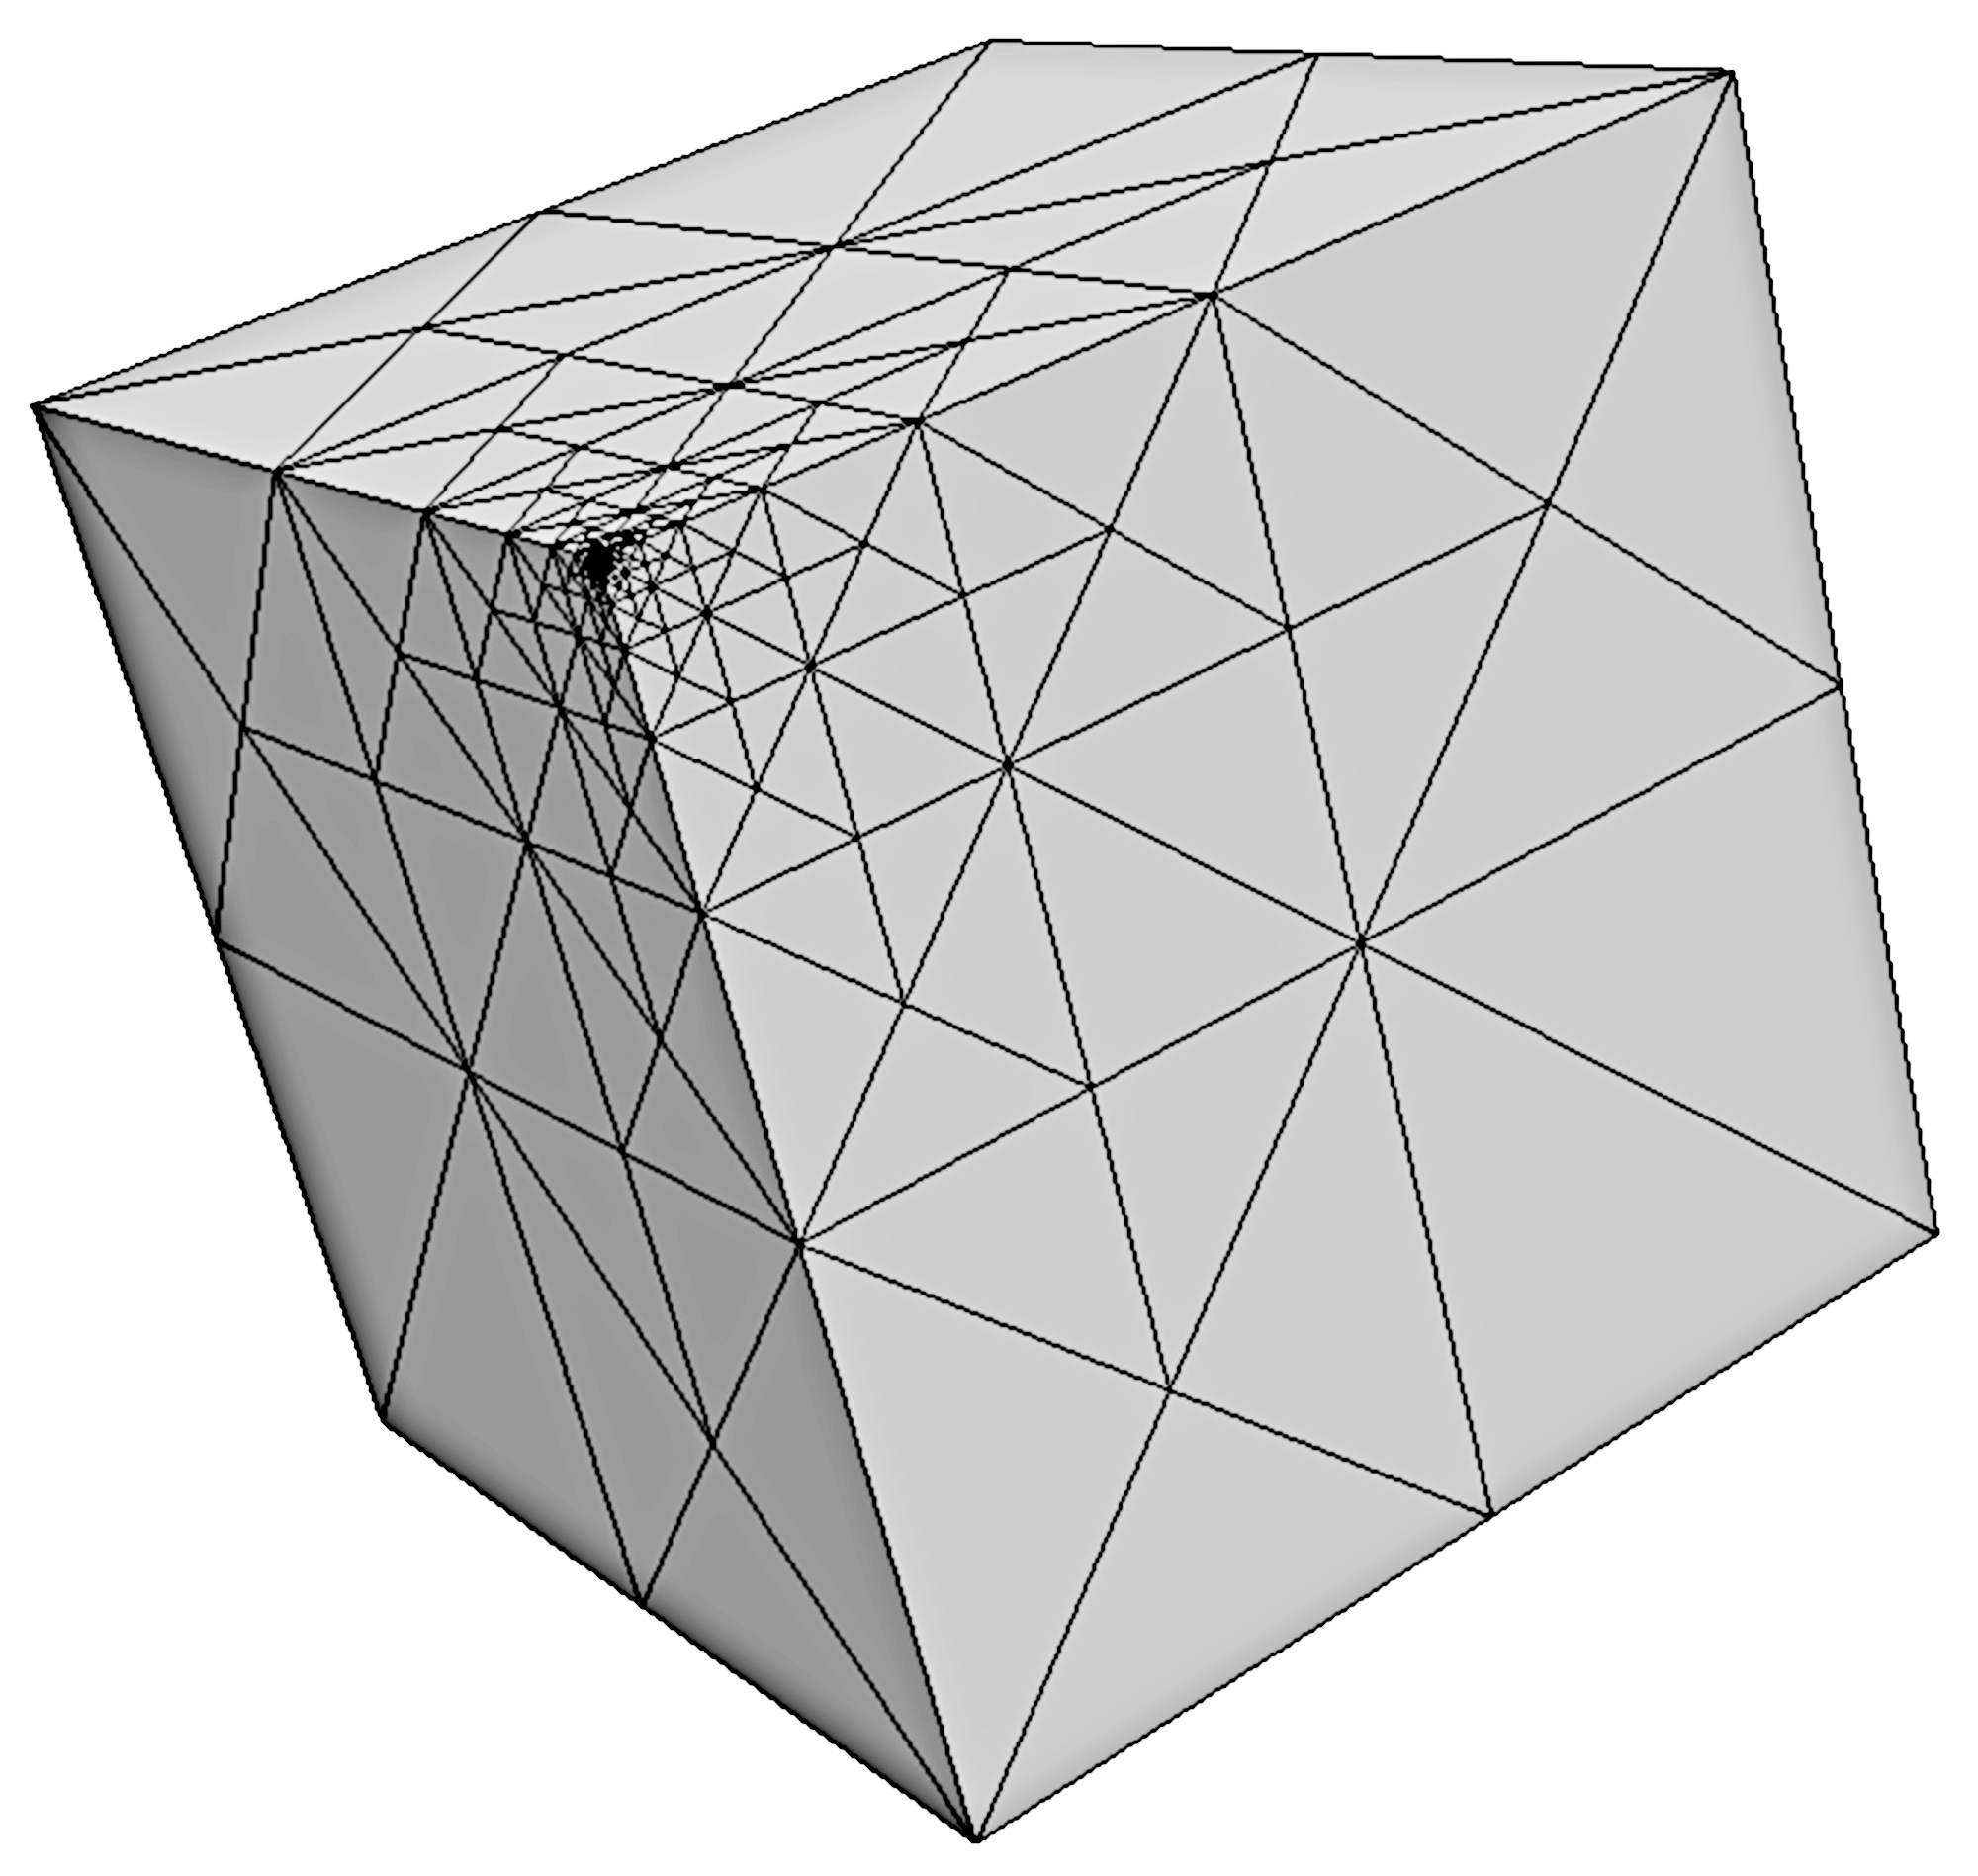
\includegraphics[width=8cm]{chapters/logg-2/png/refined_cube.png}
  \caption{A locally refined mesh obtained by repeated marking of the
    cells close to one of the corners of the unit cube.}
  \label{fig:logg-2:refinement}
\end{figure}


\paragraph{Parallel meshes.}

When running a program in parallel on a distributed memory architecture
(using MPI by invoking the program with the \emp{mpirun} wrapper),
DOLFIN automatically partitions and distributes meshes. Each process
then stores a portion of the global mesh as a standard \emp{Mesh}
object. In addition, it stores auxiliary data needed for correctly
computing local-to-global maps on each process and for communicating
data to neighboring regions. Parallel computing with DOLFIN is discussed
in Section~\ref{sec:logg-2:implementation}.

%------------------------------------------------------------------------------
\subsection{Finite elements}

The concept of a finite element as discussed in
Chapters~\ref{chap:kirby-7} and~\ref{chap:kirby-6} (the Ciarlet
definition) is implemented by the DOLFIN \emp{FiniteElement} class. This
class is implemented differently in the C++ and Python interfaces.

The C++ implementation of the \emp{FiniteElement} class relies on
code generated by a form compiler such as FFC or SFC, which are discussed
in Chapters~\ref{chap:logg-1} and~\ref{chap:alnes-3}, respectively. The
class \emp{FiniteElement} is essentially a wrapper class for the UFC class
\emp{ufc::finite\_element}. A C++ \emp{FiniteElement} provides all
the functionality of a \emp{ufc::finite\_element}. Users of the DOLFIN C++
interface will typically not use the \emp{FiniteElement} class directly,
but it is an important building block for the \emp{FunctionSpace} class, which
is discussed below. However, users developing advanced algorithms that
require run-time evaluation of finite element basis function will need
to familiarize themselves with the \emp{FiniteElement} interface. For
details, we refer to the FEniCS Programmer's Reference.

The Python interface also provides a \emp{FiniteElement} class.
The Python \emp{FiniteElement} class is
imported directly from the UFL Python module (see
Chapter~\ref{chap:alnes-1}). As such, it is just a label for a
particular finite element that can be used to define variational
problems. Variational problems are more conveniently defined in
terms of the DOLFIN \emp{FunctionSpace} class,
so users of the Python interface are rarely confronted with
the \emp{FiniteElement} class. However, advanced users who wish to
develop algorithms in Python that require functionality defined in the
UFC interface, such as run-time evaluation of basis functions, can
access such functionality by explicitly generating code from within
the Python interface. This can be accomplished by a call to the
DOLFIN \emp{jit} function (just-in-time compilation), which takes as
input a UFL \emp{FiniteElement} and returns a pair containing a
\emp{ufc::finite\_element} and a \emp{ufc::dofmap}. The returned
objects are created by first generating the corresponding C++ code,
then compiling and wrapping that C++ code into a Python module. The
returned objects are therefore directly usable from within Python.

The degrees of freedom of a \emp{FiniteElement} can be plotted directly
from the Python interface by a call to \emp{plot(element)}. This will
draw a picture of the shape of the finite element, along with a graphical
representation of its degrees of freedom in accordance with the notation
described in Chapter~\ref{chap:kirby-6}.

Table~\ref{tab:logg-2:elements} lists the finite elements currently
supported by DOLFIN (and the tool-chain FIAT--UFL--FFC/SFC--UFC). A
\emp{FiniteElement} may be specified (from Python) using either its full
name or its short symbol, as illustrated in the code example below:
%%
\begin{uflcode}
element = FiniteElement("Lagrange", tetrahedron, 5)
element = FiniteElement("CG", tetrahedron, 5)

element = FiniteElement("Brezzi-Douglas-Marini", triangle, 3)
element = FiniteElement("BDM", triangle, 3)

element = FiniteElement("Nedelec 1st kind H(curl)", tetrahedron, 2)
element = FiniteElement("N1curl", tetrahedron, 2)
\end{uflcode}

\begin{table}
  \begin{center}
    \begin{tabular}{ll}
      \toprule
      Name & Symbol \\
      \midrule
      \grey{\it Argyris} & \grey{\it ARG} \\
      \grey{\it Arnold--Winther} & \grey{\it AW} \\
      Brezzi--Douglas--Marini & BDM \\
      Crouzeix--Raviart & CR \\
      Discontinuous Lagrange & DG \\
      \grey{\it Hermite} & \grey{\it HER} \\
      Lagrange & CG \\
      \grey{\it Mardal--Tai--Winther} & \grey{\it MTW} \\
      \grey{\it Morley} & \grey{\it MOR} \\
      \nedelec{} 1st kind $\Hcurl$ & N1curl \\
      \nedelec{} 2nd kind $\Hcurl$ & N2curl \\
      Raviart--Thomas & RT \\
      \bottomrule
    \end{tabular}
    \caption{List of finite elements supported by DOLFIN~1.0. Elements
      in grey italics are partly supported in FEniCS but not
      throughout the entire tool-chain.}
    \label{tab:logg-2:elements}
  \end{center}
\end{table}

%------------------------------------------------------------------------------
\subsection{Function spaces}

The DOLFIN \emp{FunctionSpace} class represents a finite element function
space~$V_h$, as defined in Chapter~\ref{chap:kirby-7}. The data of a
\emp{FunctionSpace} is represented in terms of a triplet consisting of
a \emp{Mesh}, a \emp{DofMap} and a \emp{FiniteElement}:
%%
\vspace{0.2cm}
\begin{center}
  \emp{FunctionSpace} = (\emp{Mesh},\; \emp{DofMap},\; \emp{FiniteElement}).
\end{center}
\vspace{0.2cm}
%%
The \emp{Mesh} defines the computational domain and its
discretization. The \emp{DofMap} defines how the degrees of freedom
of the function space are distributed. In particular, the \emp{DofMap}
provides the function \emp{tabulate\_dofs} which maps the local degrees
of freedom on any given cell of the \emp{Mesh} to global degrees of
freedom. The \emp{DofMap} plays a role in defining the global regularity
of the finite element function space.  The \emp{FiniteElement} defines
the local function space on any given cell of the \emp{Mesh}. Note that
if two or more \emp{FunctionSpace}s are created on the same \emp{Mesh},
that \emp{Mesh} is shared between the two \emp{FunctionSpace}s.

\paragraph{Creating function spaces.}

As for the \emp{FiniteElement} class, \emp{FunctionSpace}s are handled
differently in the C++ and Python interfaces. In C++, the instantiation
of a \emp{FunctionSpace} relies on generated code. As an example,
we consider here the creation of a \emp{FunctionSpace} representing
continuous piecewise linear Lagrange polynomials on triangles. First,
the corresponding finite element must be defined in the UFL form
language. We do this by entering the following code into a file named
\emp{Lagrange.ufl}:
%%
\begin{uflcode}
element = FiniteElement("Lagrange", triangle, 1)
\end{uflcode}
%%
We may then generate C++ code using a form compiler such as FFC:
%%
\begin{bash}
ffc -l dolfin Lagrange.ufl
\end{bash}
This generates a file named \emp{Lagrange.h} that we may include in
our C++ program to instantiate a \emp{FunctionSpace} on a given
\emp{Mesh}:
%%
\begin{c++}
#include <dolfin.h>
#include "Lagrange.h"

using namespace dolfin;

int main()
{
  UnitSquare mesh(8, 8);
  Lagrange::FunctionSpace V(mesh);

  ...
  return 0;
}
\end{c++}
%%
In typical applications, a \emp{FunctionSpace} is not generated
through a separate \emp{.ufl} file, but is instead generated as part
of the code generation for a variational problem.

From the Python interface, one may create a \emp{FunctionSpace}
directly, as illustrated by the following code, that creates the same
function space as the above example (piecewise linear Lagrange
polynomials on triangles):

\begin{python}
mesh = UnitSquare(8, 8)
V = FunctionSpace(mesh, "Lagrange", 1)
\end{python}

\paragraph{Mixed spaces.}

Mixed function spaces may be created from arbitrary combinations of
function spaces. As an example, we consider here the creation of the
\emph{Taylor--Hood} function space for the discretization of the Stokes
or incompressible Navier--Stokes equations. This mixed function space
consists of a vector-valued continuous piecewise quadratic function space
for the velocity field and a scalar continuous piecewise linear function
space for the pressure field. This may be easily defined in either a
UFL form file (for code generation and subsequent inclusion in a C++
program) or directly in a Python script as illustrated in the following
code examples:
%%
\begin{uflcode}
V = VectorElement("CG", triangle, 2)
Q = FiniteElement("CG", triangle, 1)
W = V * Q
\end{uflcode}
%%
\begin{python}
V = VectorFunctionSpace("CG", triangle, 2)
Q = FunctionSpace("CG", triangle, 1)
W = V * Q
\end{python}

DOLFIN allows the generation of arbitrarily nested mixed function
spaces. A mixed function space can be used as a building block in the
construction of a larger mixed space. When a mixed function space is
created from more than two function spaces (nested on the same level),
then one must use the \emp{MixedElement} constructor (in UFL/C++) or
the \emp{MixedFunctionSpace} constructor (in Python). This is because
Python will interpret the expression \emp{V * Q * P} as \emp{(V *
  Q) * P}, which will create a mixed function space consisting of two
subspaces: the mixed space \emp{V * Q} and the space \emp{P}. If that is
not the intention, one must instead define the mixed function space using
\emp{MixedElement([V, Q, P])} in UFL/C++ or \emp{MixedFunctionSpace([V,
Q, P])} in Python.


\paragraph{Subspaces.}

For a mixed function space, one may access its subspaces. These
subspaces differ, in general, from the function spaces that were used to
create the mixed space in their degree of freedom maps (\emp{DofMap}
objects). Subspaces are particularly useful for applying boundary
conditions to components of a mixed element. We return to this
issue below.

%------------------------------------------------------------------------------
\subsection{Functions}

The \emp{Function} class represents a finite element
function~$u_h$ in a finite element space~$V_h$ as defined in
Chapter~\ref{chap:kirby-7}:
%%
\begin{equation}
  u_h(x) = \sum_{j=1}^N U_j \phi_j(x),
\end{equation}
%%
where $U \in \R^N$ is the vector of degrees of freedom for the
function~$u_h$ and $\{\phi_j\}_{j=1}^N$ is a basis for $V_h$.  A
\emp{Function} is represented in terms of a \emp{FunctionSpace} and a
\emp{GenericVector}:
%%
\vspace{0.2cm}
\begin{center}
  \emp{Function} = (\emp{FunctionSpace},\; \emp{GenericVector}).
\end{center}
\vspace{0.2cm}
%%
The \emp{FunctionSpace} defines the function space $V_h$ and the
\emp{GenericVector} holds the vector~$U$ of degrees of freedom; see
Figure~\ref{fig:logg-2:femsolution}. When running in parallel on a
distributed memory architecture, the \emp{FunctionSpace} and the
\emp{GenericVector} are distributed across the processes.

\begin{figure}
  \center\fenicsfig{logg-2}{femsolution}{\largefig}
  \caption{A piecewise linear finite element function~$u_h$ on a
    mesh consisting of triangular elements. The vector of degrees of
    freedom~$U$ is given by the values of~$u_h$ at the mesh
    vertices.}
  \label{fig:logg-2:femsolution}
\end{figure}

\paragraph{Creating functions.}

To create a \emp{Function} on a \emp{FunctionSpace}, one simply calls
the constructor of the \emp{Function} class with the \emp{FunctionSpace}
as the argument, as illustrated in the following code examples:
%%
\begin{c++}
Function u(V);
\end{c++}
%%
\begin{python}
u = Function(V)
\end{python}
%%
If two or more \emp{Function}s are created on the same
\emp{FunctionSpace}, the \emp{FunctionSpace} is shared between the
\emp{Function}s.

A \emp{Function} is typically used to hold the computed solution to a
partial differential equation. One may then obtain the degrees of
freedom $U$ by solving a system of equations, as illustrated in the
following code examples:
%%
\begin{c++}
Function u(V);
solve(A, u.vector(), b);
\end{c++}
%%
\begin{c++}
u = Function(V)
solve(A, u.vector(), b)
\end{c++}
%%
The process of assembling and solving a linear system is handled
automatically by the class \emp{Variational\-Problem}, which will be
discussed in more detail below.

\paragraph{Function evaluation.}

A \emp{Function} may be evaluated at arbitrary points inside the
computational domain.\footnote{One may also evaluate a \emp{Function}
  outside of the computational domain by setting the global parameter value
  \emp{"allow\_extrapolation"} to true. This may sometimes be
  necessary when evaluating a \emp{Function} on the boundary of a
  domain since round-off errors may result in points slightly outside
  of the domain.} The value of a \emp{Function} is computed by first
locating the cell of the mesh containing the given point, and then
evaluating the linear combination of basis functions on that cell. Finding
the cell exploits an efficient search tree
algorithm that is implemented as part of \citet{www:cgal}.

The following code examples illustrate function evaluation in the C++
and Python interfaces for scalar- and vector-valued functions:
%%
\begin{c++}
# Evaluation of scalar function
double scalar = u(0.1, 0.2, 0.3);

# Evaluation of vector-valued function
Array<double> vector(3);
u(vector, 0.1, 0.2, 0.3);
\end{c++}
%%
\begin{python}
# Evaluation of scalar function
scalar = u(0.1, 0.2, 0.3)

# Evaluation of vector-valued function
vector = u(0.1, 0.2, 0.3)
\end{python}
%%
When running in parallel with a distributed mesh, functions can only be
evaluated at points located in the portion of the mesh that is stored
by the local process.

\paragraph{Subfunctions.}

For \emp{Function}s constructed on a mixed \emp{FunctionSpace},
subfunctions (components) of the \emp{Function} can be accessed, for
example to plot the solution components of a mixed system. Subfunctions
may be accessed as either \emph{shallow} or \emph{deep copies}. By
default, subfunctions are accessed as shallow copies, which means that
the subfunctions share data with their parent functions.  They provide
\emph{views} to the data of the parent function. Sometimes, it may also be
desirable to access subfunctions as deep copies. A deep copied subfunction
does not share its data (namely, the vector holding the degrees of
freedom) with the parent \emp{Function}.  Both shallow and deep copies
of \emp{Function} objects are themselves \emp{Function} objects and may
(with some exceptions) be used as regular \emp{Function} objects.

Creating shallow and deep copies of subfunctions is done
differently in C++ and Python, as illustrated by the following code
examples:
%%
\begin{c++}
Function w(W);

// Create shallow copies
Function& u = w[0];
Function& p = w[1];

// Create deep copies
Function uu = w[0];
Function pp = w[1];
\end{c++}
%%
\begin{python}
w = Function(W)

# Create shallow copies
u, p = w.split()

# Create deep copies
uu, pp = w.split(deepcopy=True)
\end{python}
%%
Note that component access, such as \emp{w[0]}, from the Python
interface does not create a new \emp{Function} object as in the C++
interface. Instead, it creates a UFL expression that denotes a
component of the original \emp{Function}.

%------------------------------------------------------------------------------
\subsection{Expressions}

The \emp{Expression} class is closely related to the \emp{Function}
class in that it represents a function that can be evaluated on a
finite element space. However, where a \emp{Function} must be defined
in terms of a vector of degrees of freedom, an \emp{Expression} may be
freely defined in terms of, for example, coordinate values, other
geometric entities, or a table lookup.

An \emp{Expression} may be defined in both C++ and Python by
subclassing the \emp{Expression} class and overloading the \emp{eval}
function, as illustrated in the following code examples which define
the function $f(x, y) = \sin x \, \cos y$ as an \emp{Expression}:
%%
\begin{c++}
class MyExpression : public Expression
{
  void eval(Array<double>& values, const Array<double>& x) const
  {
    values[0] = sin(x[0])*cos(x[1]);
  }
};

MyExpression f;
\end{c++}
%%
\begin{python}
class MyExpression(Expression):
    def eval(self, values, x):
        values[0] = sin(x[0])*cos(x[1])

f = MyExpression()
\end{python}
%%
For vector-valued (or tensor-valued) \emp{Expression}s, one must also
specify the value shape of the \emp{Expression}. The following code
examples demonstrate how to implement the vector-valued function $g(x,
y) = (\sin x, \cos y)$. The value shape is defined slightly
differently in C++ and Python.
%%
\begin{c++}
class MyExpression : public Expression
{
  void eval(Array<double>& values, const Array<double>& x) const
  {
    values[0] = sin(x[0]);
    values[1] = cos(x[1]);
  }

  uint value_rank() const
  {
    return 1;
  }

  uint value_dimension(uint i) const
  {
    return 2;
  }
};

MyExpression g;
\end{c++}
%%
\begin{python}
class MyExpression(Expression):

    def eval(self, values, x):
        values[0] = sin(x[0])
        values[1] = cos(x[1])

    def value_shape(self):
        return (2,)

g = MyExpression()
\end{python}

The above \emph{functor} construct for the definition of expressions is
powerful and allows a user to define complex expressions, the evaluation
of which may involve arbitrary operations as part of the \emp{eval}
function. For simple expressions like $f(x, y) = \sin x \, \cos y$ and
$g(x, y) = (\sin x, \cos y)$, users of the Python interface may use a
simple syntax to define expressions:
%%
\begin{python}
f = Expression("sin(x[0]) * cos(x[1])")
g = Expression(("sin(x[0])", "cos(x[1])"))
\end{python}
%%
The above code will automatically generate subclasses of the DOLFIN C++
\emp{Expression} class that overload the \emp{eval} function. This has the
advantage of being more efficient, since the callback to the \emp{eval}
function takes place in C++ rather than in Python.

A feature that can be used to implement a time-dependent \emp{Expression}
in the Python interface is to use a variable name in an \emp{Expression}
string.  For example, one may use the variable \emp{t} to denote time:
%%
\begin{python}
h = Expression("t * sin(x[0]) * cos(x[1])")
while t < T:
    h.t = t
    ...
    t += dt
\end{python}
%%
The \emp{t} variable has here been used to create a time-dependent
\emp{Expression}. Arbitrary variable names may be used as long as they
do not conflict with the names of built-in functions, such as \emp{sin}
or~\emp{exp}.

In addition to the above examples, the Python interface allows
the direct definition of (more complex) subclasses of the C++
\emp{Expression} class by supplying C++ code for their definition. For
more information, we refer to the DOLFIN Programmer's Reference.

%------------------------------------------------------------------------------
\subsection{Variational forms}

DOLFIN relies on the FEniCS tool-chain FIAT--UFL--FFC/SFC--UFC for the
evaluation of finite element variational forms. Variational forms
expressed in the UFL form language (Chapter~\ref{chap:alnes-1})
are compiled using one of the form compilers FFC or SFC
(Chapters~\ref{chap:logg-1} and~\ref{chap:alnes-3}), and the generated
UFC code (Chapter~\ref{chap:alnes-2}) is used by DOLFIN to
evaluate (assemble) variational forms.

The UFL form language allows a wide range of variational forms to be
expressed in a language close to the mathematical notation, as exemplified
by the following expressions defining (in part) the bilinear and linear
forms for the discretization of a linear elastic problem:
%%
\begin{uflcode}
a = inner(sigma(u), epsilon(v))*dx
L = dot(f, v)*dx
\end{uflcode}
%%
This should be compared to the corresponding mathematical notation:
%%
\begin{align} \label{eq:logg-2:elasticity1}
  a(u, v) &= \int_{\Omega} \sigma(u) : \epsilon(v) \dx,
\\
  L(v)    &= \int_{\Omega} f \cdot v \dx.
\end{align}
%%
Here, $\epsilon(v) = (\nabla v + (\nabla v)^{T}) / 2$ denotes the
symmetric gradient and $\sigma(v) = 2 \mu \, \epsilon(v) + \lambda
\mathrm{tr} \, \epsilon(v) I$ is the stress tensor. For a detailed
presentation of the UFL form language, we refer to
Chapter~\ref{chap:alnes-1}.

The code generation process must be handled explicitly by users of the C++
interface by calling a form compiler on the command-line. To solve the
linear elastic problem above for a specific choice of parameter values
(the Lam\'e constants~$\mu$ and~$\lambda$), a user may enter the following
code in a file named \emp{Elasticity.ufl}\footnote{Note that `lambda'
has been deliberately misspelled since it is a reserved keyword
in Python.}:
%%
\begin{uflcode}
V = VectorElement("Lagrange", tetrahedron, 1)

u = TrialFunction(V)
v = TestFunction(V)
f = Coefficient(V)

E  = 10.0
nu = 0.3

mu    = E/(2.0*(1.0 + nu))
lmbda = E*nu/((1.0 + nu)*(1.0 - 2.0*nu))

def sigma(v):
    return 2.0*mu*sym(grad(v)) + lmbda*tr(sym(grad(v)))*Identity(v.cell().d)

a = inner(sigma(u), sym(grad(v)))*dx
L = dot(f, v)*dx
\end{uflcode}
%%
This code may be compiled using a UFL/UFC compliant form compiler to
generate UFC C++ code. For example, using FFC:
%%
\begin{bash}
ffc -l dolfin Elasticity.ufl
\end{bash}
%%
This generates a C++ header file (including implementation) named
\emp{Elasticity.h} which may be included in a C++ program and used to
instantiate the two forms~\emp{a} and~\emp{L}:
%%
\begin{c++}
#include <dolfin.h>
#include "Elasticity.h"

using namespace dolfin;

int main()
{
  UnitSquare mesh(8, 8);
  Elasticity::FunctionSpace V(mesh);
  Elasticity::BilinearForm a(V, V);
  Elasticity::LinearForm L(V);
  MyExpression f; // code for the definition of MyExpression omitted
  L.f = f;

  return 0;
}
\end{c++}
%%
The instantiation of the forms involves the instantiation of the
\emp{FunctionSpace} on which the forms are defined. Any coefficients
appearing in the definition of the forms (here the right-hand side
\emp{f}) must be attached after the creation of the forms.

Python users may rely on automated code generation, and define variational
forms directly as part of a Python script:
%%
\begin{python}
from dolfin import *

mesh = UnitSquare(8, 8)
V = VectorElement("Lagrange", tetrahedron, 1)

u = TrialFunction(V)
v = TestFunction(V)
f = MyExpression() # code emitted for the definition of f

E  = 10.0
nu = 0.3

mu    = E/(2.0*(1.0 + nu))
lmbda = E*nu/((1.0 + nu)*(1.0 - 2.0*nu))

def sigma(v):
    return 2.0*mu*sym(grad(v)) + lmbda*tr(sym(grad(v)))*Identity(v.cell().d)

a = inner(sigma(u), sym(grad(v)))*dx
L = dot(f, v)*dx
\end{python}
%%
This script will trigger automatic code generation for the definition
of the \emp{FunctionSpace}~\emp{V}. Code generation of the two
forms~\emp{a} and~\emp{L} is postponed until the point when the
corresponding discrete operators (the matrix and vector) are
assembled.

%------------------------------------------------------------------------------
\subsection{Finite element assembly}

A core functionality of DOLFIN is the assembly of finite element
variational forms. Given a variational form (\emp{a}), DOLFIN assembles
the corresponding discrete operator~(\emp{A}). The assembly of the
discrete operator follows the general algorithm described in
Chapter~\ref{chap:logg-3}. The following code illustrates how to
assemble a scalar (\emp{m}), a vector (\emp{b}) and a matrix (\emp{A})
from a functional (\emp{M}), a linear form (\emp{L}) and a bilinear
form (\emp{a}), respectively:
%%
\begin{c++}
Vector b;
Matrix A;

double m = assemble(M);
assemble(b, L);
assemble(A, a);
\end{c++}
%%
\begin{python}
m = assemble(M)
b = assemble(L)
A = assemble(a)
\end{python}
%%
The assembly of variational forms from the Python interface
automatically triggers code generation, compilation and linking at
run-time. The generated code is automatically instantiated and sent to
the DOLFIN C++ compiler. As a result, finite element assembly from the
Python interface is equally efficient as assembly from the C++
interface, with only a small overhead for handling the automatic code
generation. The generated code is cached for later reuse, hence
repeated assembly of the same form or running the same program twice
does not re-trigger code generation. Instead, the previously generated
code is automatically loaded.

DOLFIN provides a common assembly algorithm for the assembly of tensors
of any rank (scalars, vectors, matrices, \ldots) for any form. This is
possible since the assembly algorithm relies on the \emp{GenericTensor}
interface, portions of the assembly algorithm that depend on the
variational form and its particular discretization are generated prior to
assembly, and the mesh interface is dimension-independent.  The assembly
algorithm accepts a number of optional arguments that control whether
the sparsity of the assembled tensor should be reset before assembly
and whether the tensor should be zeroed before assembly. Arguments may
also be supplied to specify subdomains of the \emp{Mesh} if the form is
defined over particular subdomains (using \emp{dx(0)}, \emp{dx(1)} etc.).

In addition to the \emp{assemble} function, DOLFIN provides the
\emp{assemble\_system} function which assembles a pair of forms
consisting of a bilinear and a linear form and applies essential
boundary conditions during the assembly process. The application of
boundary conditions as part of the call to \emp{assemble\_system}
preserves symmetry of the matrix being assembled (see
Chapter~\ref{chap:logg-3}).

The assembly algorithms have been parallelized for both distributed
memory architectures (clusters) using MPI and shared memory
architectures (multi-core) using OpenMP. This is discussed in more detail in
Section~\ref{sec:logg-2:implementation}.

%------------------------------------------------------------------------------
\subsection{Boundary conditions}

DOLFIN handles the application of both Neumann (natural) and Dirichlet
(essential) boundary conditions.\footnote{As noted in
  Chapter~\ref{chap:kirby-7}, Dirichlet boundary conditions may
  sometimes be \emph{natural} and Neumann boundary conditions may
  sometimes be \emph{essential}.} Natural boundary are usually applied
via the variational statement of a problem, whereas essential boundary
conditions are usually applied to the discrete system of equations.

\paragraph{Natural boundary conditions.}

Natural boundary conditions typically appear as boundary terms as the
result of integrating by parts a partial differential equation multiplied
by a test function. As a simple example, we consider the linear elastic
variational problem. The partial differential equation governing the
displacement of an elastic body may be expressed as
%%
\begin{equation} \label{eq:logg-2:elasticity}
  \begin{array}{rcll}
    - \nabla \cdot \sigma(u) &=& f \quad &\mbox{in } \Omega,
    \\
    \sigma n &=& g \quad  &\mbox{on } \Gamma_{\mathrm{N}} \subset \partial\Omega,
    \\
    u &=& u_0 \quad  &\mbox{on } \Gamma_{\mathrm{D}} \subset \partial\Omega,
    \end{array}
\end{equation}
%%
where $u$ is the unknown displacement field to be computed,
$\sigma(u)$ is the stress tensor, $f$ is a given body force, $g$ is a
given traction on a portion $\Gamma_{\mathrm{N}}$ of the boundary, and
$u_0$ is a given displacement on a portion $\Gamma_{\mathrm{D}}$ of
the boundary. Multiplying by a test function $v$ and integrating by
parts, we obtain
%%
\begin{equation}
  \int_{\Omega} \sigma(u) : \epsilon(v) \dx - \int_{\partial\Omega}
  \sigma n \cdot v \ds = \int_{\Omega} f \cdot v \dx,
\end{equation}
%%
where we have used the symmetry of $\sigma(u)$ to replace $\nabla v$
by the symmetric gradient $\epsilon(v)$. Since the displacement~$u$
is known on the Dirichlet boundary $\Gamma_{\mathrm{D}}$, we let $v =
0$ on~$\Gamma_{\mathrm{D}}$. Furthermore, we replace $\sigma n$ by the
given traction~$g$ on the remaining (Neumann) portion of the boundary
$\Gamma_{\mathrm{N}}$ to obtain
%%
\begin{equation}
  \int_{\Omega} \sigma(u) : \epsilon(v) \dx
    = \int_{\Omega} f \cdot v \dx + \int_{\Gamma_{\mathrm{N}}} g \cdot v \ds.
\end{equation}
%%
The following code demonstrates how to implement this variational
problem in the UFL form language, either as part of a \emp{.ufl} file
or as part of a Python script:
%%
\begin{uflcode}
a = inner(sigma(u), sym(grad(v)))*dx
L = dot(f, v)*dx + dot(g, v)*ds
\end{uflcode}

To specify that the boundary integral \emp{dot(g, v)*ds} should only
be evaluated along the Neumann boundary $\Gamma_{\mathrm{N}}$, one
must specify which part of the boundary is included in the \emp{ds}
integral. An easy way to accomplish this is to specify~\emp{g} in such
a way that it is zero on the Neumann boundary. In cases where this is
not convenient, one must instead specify the Neumann boundary in terms
of a \emp{FacetFunction}. This \emp{FacetFunction} must specify for
each facet of the \emp{Mesh} to which part of the boundary it
belongs. For the current example, an appropriate strategy is to mark
each facet on the Neumann boundary by~\emp{0} and all other facets
(including facets internal to the domain) by~\emp{1}. This can be
accomplished in a number of different ways. One simple way to do this
is to use the program \citet{www:meshbuilder} and graphically mark the
facets of the \emp{Mesh}. Another option is through the DOLFIN class
\emp{SubDomain}. The following code illustrates how to mark all facets
to the left of $x = 0.5$ as the Neumann boundary. Note the use of the
\emp{on\_boundary} argument supplied by DOLFIN to the \emp{inside}
function. This argument informs whether a point is located on the
boundary $\partial\Omega$ of $\Omega$, and this allows us to mark only
facets that are on the boundary and to the left of~$x = 0.5$. Also
note the use of \emp{DOLFIN\_EPS} which makes sure that we include
points that, as a result of finite precision arithmetic, may be located
just to the right of $x = 0.5$.
%%
\begin{c++}
class NeumannBoundary : public SubDomain
{
  bool inside(const Array<double>& x, bool on_boundary) const
  {
    return x[0] < 0.5 + DOLFIN_EPS && on_boundary;
  }
};

NeumannBoundary neumann_boundary;
FacetFunction<uint> exterior_facet_domains(mesh, 1);
neumann_boundary.mark(exterior_facet_domains, 0);
\end{c++}
%%
\begin{python}
class NeumannBoundary(SubDomain):
    def inside(self, x, on_boundary):
        return x[0] < 0.5 + DOLFIN_EPS and on_boundary

neumann_boundary = NeumannBoundary()
exterior_facet_domains = FacetFunction("uint", mesh, 1)
neumann_boundary.mark(exterior_facet_domains, 0)
\end{python}
%%
The correct specification of boundaries is a common error source. For
debugging the specification of boundary conditions, it can be helpful
to plot the \emp{FacetFunction} that specifies the boundary markers by
writing the \emp{FacetFunction} to a VTK file (see the file I/O section)
or using the \emp{plot} command. When using the \emp{plot} command,
the plot shows the facet values interpolated to the vertices of the
\emp{Mesh}. As a result, care must be taken to interpret the plot close
to domain boundaries (corners) in this case. The issue is not present
in the VTK output.

In the above example, we mark the Neumann boundary by~\emp{0}. This is
appropriate since in the UFL form language, \emp{ds} is the same as
\emp{ds(0)}. The default domain of integration is the domain marked
by~\emp{0}. One could also have used \emp{ds(1)} and marked the
Neumann boundary by~\emp{1}.

\paragraph{Essential boundary conditions.}

The application of essential boundary conditions is handled by the
class \emp{DirichletBC}. Using this class, one may specify a Dirichlet
boundary condition in terms of a \emp{FunctionSpace}, a \emp{Function}
or an \emp{Expression}, and a subdomain. The subdomain may be
specified either in terms of a \emp{SubDomain} object or in terms of a
\emp{FacetFunction}. A \emp{DirichletBC} specifies that the solution
should be equal to the given value on the given subdomain.

The following code examples illustrates how to define the Dirichlet
condition $u(x) = u_0(x) = \sin x$ on the Dirichlet boundary
$\Gamma_{\mathrm{D}}$ (assumed here to be the part of the boundary
to the right of $x = 0.5$) for the elasticity
problem~\eqref{eq:logg-2:elasticity} using the \emp{SubDomain}
class. Alternatively, the subdomain may be specified using a
\emp{FacetFunction}.
%%
\begin{c++}
class DirichletValue : public Expression
{
  void eval(Array<double>& values, const Array<double>& x) const
  {
    values[0] = sin(x[0]);
  }
};

class DirichletBoundary : public SubDomain
{
  bool inside(const Array<double>& x, bool on_boundary) const
  {
    return x[0] > 0.5 - DOLFIN_EPS && on_boundary;
  }
};

DirichletValue u_0;
DirichletBoundary Gamma_D;

DirichletBC bc(V, u_0, Gamma_D);
\end{c++}
%%
\begin{python}
class DirichletValue(Expression):
    def eval(self, value, x):
        values[0] = sin(x[0])

class DirichletBoundary(SubDomain):
    def inside(self, x, on_boundary):
        return x[0] > 0.5 - DOLFIN_EPS and on_boundary

u_0 = DirichletValue()
Gamma_D = DirichletBoundary()

bc = DirichletBC(V, u_0, Gamma_D)
\end{python}
%%
Python users may also use the following compact syntax:
%%
\begin{python}
def Gamma_D(x, on_boundary):
    return x[0] > 0.5 and on_boundary

u_0 = Expression("sin(x[0])")

bc = DirichletBC(V, u_0, Gamma_D)
\end{python}
%%
To speed up the application of Dirichlet boundary conditions, users of the
Python interface may also use the function \emp{compile\_subdomains}. For
details of this, we refer to the DOLFIN Programmer's reference.

A Dirichlet boundary condition can be applied to a linear system or to
a vector of degrees of freedom associated with a \emp{Function}, as
illustrated by the following code examples:
%%
\begin{c++}
bc.apply(A, b);
bc.apply(u.vector());
\end{c++}
%%
\begin{python}
bc.apply(A, b)
bc.apply(u.vector())
\end{python}
%%
The application of a Dirichlet boundary condition to a linear system
will identify all degrees of freedom that should be set to the given
value and modify the linear system such that its solution respects the
boundary condition. This is accomplished by zeroing and inserting~$1$
on the diagonal of the rows of the matrix corresponding to Dirichlet
values, and inserting the Dirichlet value in the corresponding entry
of the right-hand side vector. This application of boundary conditions
does not preserve symmetry. If symmetry is required, one may
alternatively consider using the \emp{assemble\_system} function which
applies Dirichlet boundary conditions symmetrically as part of the
assembly process.

Multiple boundary conditions may be applied to a single system or
vector. If two different boundary conditions are applied to the same
degree of freedom, the last applied value will overwrite any
previously set values.

%------------------------------------------------------------------------------
\subsection{Variational problems}

Variational problems (finite element discretizations of partial
differential equations) can be easily solved in DOLFIN using the class
\emp{VariationalProblem}. This is done by first specifying a
\emp{VariationalProblem} in terms of a pair of forms and (possibly)
boundary conditions, and then calling the \emp{solve} member function.

Both linear and nonlinear problems can be solved. A linear problem
must be expressed in the following canonical form: find $u \in V$ such
that
%%
\begin{equation}
  a(u, v) = L(v) \quad \foralls v \in \hat{V}.
\end{equation}
A nonlinear problem must be expressed in the following canonical form:
find $u \in V$ such that
%%
\begin{equation}
  F(u; v) = 0 \quad \foralls v \in \hat{V}.
\end{equation}
%%
In the case of a linear variational problem specified in terms of a
bilinear form~\emp{a} and a linear form~\emp{L}, the solution is
computed by assembling the matrix~\emp{A} and vector~\emp{b} of the
corresponding linear system, then applying boundary conditions to the
system, and finally solving the linear system. In the case of a
nonlinear variational problem specified in terms of a linear
form~\emp{F} and a bilinear form~\emp{dF} (the derivative or Jacobian
of~\emp{F}), the solution is computed by Newton's method. DOLFIN
determines whether a problem is linear or nonlinear based on the given
forms; if a pair of bilinear and linear forms (\emp{a} and \emp{L})
are given, then the problem is assumed to be linear, and if a pair of
linear and bilinear forms (\emp{F} and \emp{dF}) are given, then the
problem is assumed to be nonlinear.

The code examples below demonstrate how to solve a linear variational
problem specified in terms of a bilinear form~\emp{a}, a linear
form~\emp{L} and a list of Dirichlet boundary conditions given as
\emp{DirichletBC} objects:
%%
\begin{c++}
std::vector<const BoundaryCondition*> bcs;
bcs.push_back(&bc0);
bcs.push_back(&bc1);
bcs.push_back(&bc2);

VariationalProblem problem(a, L, bcs);
Function u(V);
problem.solve(u);
\end{c++}
%%
\begin{python}
bcs = [bc0, bc1, bc2]

problem = VariationalProblem(a, L, bcs)
u = problem.solve()
\end{python}

To solve a nonlinear variational problem, one must supply both a linear
form~\emp{F} and its derivative~\emp{dF}, which is a bilinear form. In
many cases, the derivative can be easily computed using the function
\emp{derivative}, either in a \emp{.ufl} form file or as part of a Python
script. We here demonstrate how a nonlinear problem may be solved using
the Python interface:
%%
\begin{python}
u  = Function(V)
du = TrialFunction(V)
v  = TestFunction(V)
F  = inner((1 + u**2)*grad(u), grad(v))*dx - f*v*dx
dF = derivative(F, u, du)

problem = VariationalProblem(F, dF, bcs)
problem.solve(u)
\end{python}

A \emp{VariationalProblem} provides a range of parameters that can be
adjusted to control the solution process. To view the list of available
parameters for a \emp{VariationalProblem} object \emp{problem}, issue
the command \emp{info(problem, true)} from C++ or \emp{info(problem,
True)} from Python.

%------------------------------------------------------------------------------
\subsection{File I/O and visualization}

\paragraph{Preprocessing.}

DOLFIN has capabilities for mesh generation only in the form of the
built-in meshes \emp{UnitSquare}, \emp{UnitCube}, etc.  External software
must be used to generate more complicated meshes. To simplify this
process, DOLFIN provides a simple script \emp{dolfin-convert} to convert
meshes from other formats to the DOLFIN XML format. Currently supported
file formats are listed in Table~\ref{tab:logg-2:conversionformats}. The
following code illustrates how to convert a mesh from the Gmsh format
(suffix \emp{.msh} or \emp{.gmsh}) to the DOLFIN XML format:
%%
\begin{bash}
dolfin-convert mesh.msh mesh.xml
\end{bash}
%%
Once a mesh has been converted to the DOLFIN XML file format, it can be
read into a program, as illustrated by the following code examples:
%%
\begin{c++}
Mesh mesh("mesh.xml");
\end{c++}
%%
\begin{python}
mesh = Mesh("mesh.xml")
\end{python}

\begin{table}
  \begin{center}
    \begin{tabular}{ll}
      \toprule
      Suffix & File format \\
      \midrule
      \emp{.xml}               & DOLFIN XML format \\
      \emp{.ele} / \emp{.node} & Triangle file format \\
      \emp{.mesh}              & Medit format, generated by TetGen with option \emp{-g} \\
      \emp{.msh} / \emp{.gmsh} & Gmsh version 2.0 format \\
      \emp{.grid}              & Diffpack tetrahedral grid format \\
      \emp{.inp}               & Abaqus tetrahedral grid format \\
      \emp{.e} / \emp{.exo}    & Sandia Exodus II file format \\
      \emp{.ncdf}              & ncdump'ed Exodus II file format \\
      \emp{.vrt}/\emp{.cell}   & Star-CD tetrahedral grid format \\
      \bottomrule
    \end{tabular}
    \caption{List of file formats supported by the
      \emp{dolfin-convert} script.}
    \label{tab:logg-2:conversionformats}
  \end{center}
\end{table}

\paragraph{Postprocessing.}

To visualize a solution (\emp{Function}), a \emp{Mesh} or a
\emp{MeshFunction}, the \emp{plot} command\footnote{The plot command
  requires a working installation of the \emp{viper} Python
  module. Plotting finite elements requires access to the \emp{ffc}
  plotting module.} can be issued, from either C++ or Python:
%%
\begin{c++}
plot(u);
plot(mesh);
plot(mesh_function);
\end{c++}
%%
\begin{python}
plot(u)
plot(mesh)
plot(mesh_function)
\end{python}
%%
Example plots generated using the \emp{plot} command are presented in
Figures~\ref{fig:logg-2:plots,mesh} and~\ref{fig:logg-2:plots,function}.

\begin{figure}
  \center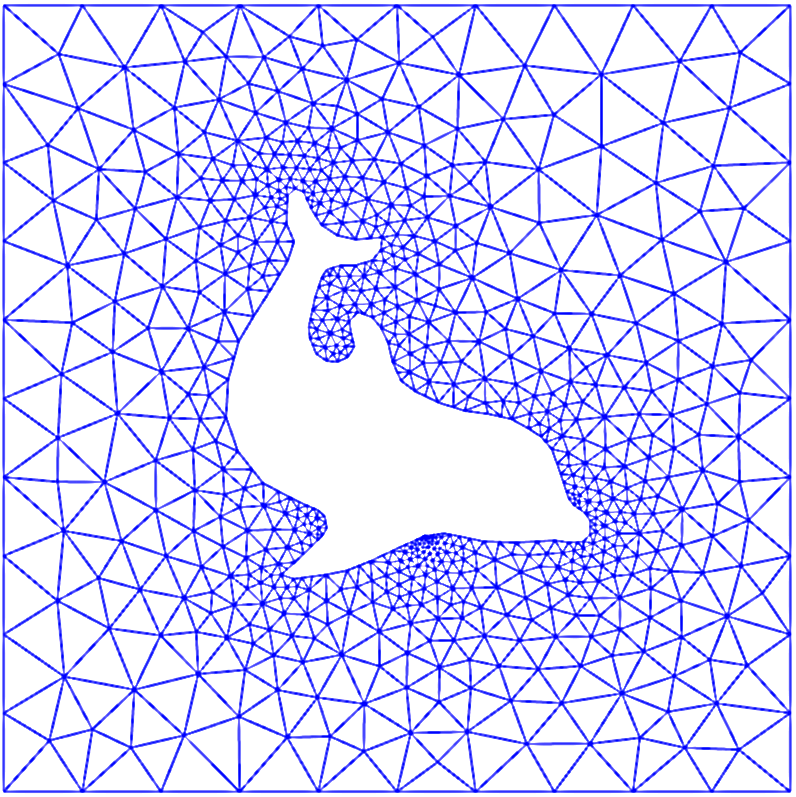
\includegraphics[width=\smallfig]{chapters/logg-2/png/plot_mesh.png}
  \caption{Plotting a mesh using the DOLFIN \emp{plot} command, here
    the mesh \emp{dolfin-1.xml.gz} distributed with DOLFIN.}
    \label{fig:logg-2:plots,mesh}
\end{figure}

\begin{figure}
  \center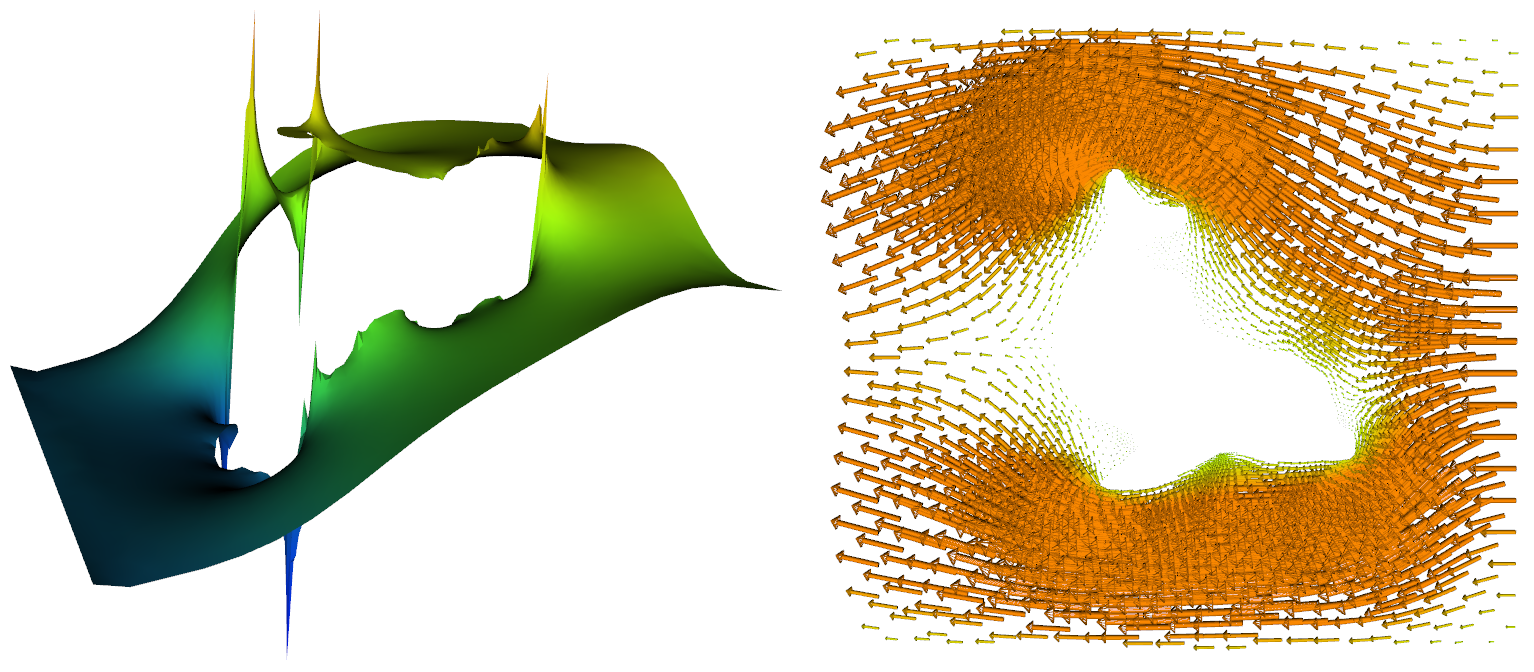
\includegraphics[width=\largefig]{chapters/logg-2/png/plots.png}
    \caption{Plotting a scalar and a vector-valued function using the
      DOLFIN \emp{plot} command, here the pressure (left) and velocity
      (right) from a solution of the Stokes equations on the mesh from
    Figure~\ref{fig:logg-2:plots,mesh}.}
    \label{fig:logg-2:plots,function}
\end{figure}

From Python, one can also plot expressions and finite elements:
%%
\begin{python}
plot(u)
plot(grad(u))
plot(u*u)

element = FiniteElement("BDM", tetrahedron, 3)
plot(element)
\end{python}
%%
To enable interaction with a plot window (rotate, zoom) from Python,
call the function \emp{interactive}, or add an optional argument
\emp{interactive=True} to the \emp{plot} command.

The \emp{plot} command provides rudimentary plotting, and advanced
postprocessing is better handled by external software such as
\citet{www:paraview} and \citet{www:mayavi}. This is easily
accomplished by storing the solution (a \emp{Function} object) to file
in PVD format (ParaView Data, an XML-based format). This can be done
in both C++ and Python by writing to a file with the \emp{.pvd}
extension, as illustrated in the following code examples:
%%
\begin{c++}
File file("solution.pvd");
file << u;
\end{c++}
%%
\begin{python}
file = File("solution.pvd")
file << u
\end{python}
%%
The standard PVD format is ASCII based, hence the file size can
become very large for large data sets. To use a compressed binary
format, a string \emp{"compressed"} can be used when creating a
PVD-based \emp{File} object:
%%
\begin{c++}
File file("solution.pvd", "compressed");
\end{c++}
%%
If multiple \emp{Function}s are written to the same file (by repeated
use of \emp{<{}<}), then the data is interpreted as a time series,
which may then be animated in ParaView or MayaVi2. Each frame of the
time series is stored as a \emp{.vtu} (VTK unstructured data) file,
with references to these files stored in the \emp{.pvd} file.  When
writing time-dependent data, it can be useful to store the time
\emp{t} of each snapshot. This is done as illustrated below:
%%
\begin{c++}
File file("solution.pvd", "compressed");
file << std::make_pair<const Function*, double>(&u, t);
\end{c++}
%%
\begin{python}
file = File("solution.pvd", "compressed");
file << (u, t)
\end{python}
%%
Storing the time is particularly useful when animating simulations that
use a varying time step.

The PVD format supports parallel post-processing. When running in
parallel, a single \emp{.pvd} file is created and a \emp{.vtu} file is
created for the data on each partition. Results computed in parallel
can be viewed seamlessly using ParaView.


\paragraph{DOLFIN XML format.}

DOLFIN XML is the native format of DOLFIN. An advantage of XML is that
it is a robust and human-readable format. If the files are compressed,
there is also little overhead in terms of file size compared to a
binary format.

Many of the classes in DOLFIN can be written to and from DOLFIN XML
files using the standard stream operators \emp{<{}<} and \emp{>{}>}, as
illustrated in the following code examples:
%%
\begin{c++}
File vector_file("vector.xml");
vector_file << vector;
vector_file >> vector;

File matrix_file("matrix.xml");
matrix_file << matrix;
matrix_file >> matrix;

File mesh_file("mesh.xml");
mesh_file << mesh;
mesh_file >> mesh;

File parameters_file("parameters.xml");
parameters_file << parameters;
parameters_file >> parameters;
\end{c++}
%%
\begin{python}
vector_file = File("vector.xml")
vector_file << vector
vector_file >> vector

matrix_file = File("matrix.xml")
matrix_file << matrix
matrix_file >> matrix

mesh_file = File("mesh.xml")
mesh_file << mesh
mesh_file >> mesh

parameters_file = File("parameters.xml")
parameters_file << parameters
parameters_file >> parameters
\end{python}
%%
One cannot read/write \emp{Function} and \emp{FunctionSpace} objects
since the representation of a \emp{FunctionSpace} (and thereby the
representation of a \emp{Function}) relies on generated code.

DOLFIN automatically handles \emph{reading} of gzipped XML files. Thus,
one may save space by storing meshes and other data in gzipped XML files
(with suffix \emp{.xml.gz}).


\paragraph{Time-series.}

For time-dependent problems, it may be useful to store a
sequence of solutions or meshes in a format that enables fast
reading/writing of data. For this purpose, DOLFIN provides the
\emp{TimeSeries} class. This enables the storage of a series of
\emp{Vector}s (of degrees of freedom) and/or \emp{Mesh}es. The
following code illustrates how to store a series of \emp{Vector}s and
\emp{Mesh}es to a \emp{TimeSeries}:
%%
\begin{c++}
TimeSeries time_series("simulation_data");

while (t < T)
{
  ...
  time_series.store(u.vector(), t);
  time_series.store(mesh, t);
  t += dt;
}
\end{c++}
%%
\begin{python}
time_series = TimeSeries("simulation_data")

while t < T:
    ...
    time_series.store(u.vector(), t)
    time_series.store(mesh, t)
    t += dt
\end{python}
%%
Data in a \emp{TimeSeries} are stored in a binary format with one
file for each stored dataset (\emp{Vector} or \emp{Mesh}) and a common
index. Data may be retrieved from a \emp{TimeSeries} by calling the
\emp{retrieve} member function as illustrated in the code examples
below. If a dataset is not stored at the requested time, then the data
is interpolated linearly for \emp{Vector}s. For \emp{Mesh}es, the
closest data point will be used.
%%
\begin{c++}
time_series.retrieve(u.vector(), t);
time_series.retrieve(mesh, t);
\end{c++}
%%
\begin{python}
time_series.retrieve(u.vector(), t);
time_series.retrieve(mesh, t);
\end{python}

%------------------------------------------------------------------------------
\subsection{Logging / diagnostics}

DOLFIN provides a simple interface for the uniform handling of log
messages, including warnings and errors. All messages are collected to a
single stream, which allows the destination and formatting of the output
from an entire program, including the DOLFIN library, to be controlled
by the user.

\paragraph{Printing messages.}

Informational messages from DOLFIN are normally printed using the
\emp{info} command. This command takes a string argument and an
optional list of variables to be formatted, much like the standard
C \emp{printf} command. Note that the \emp{info} command
automatically appends a newline to the given string. Alternatively,
C++ users may use the \emp{dolfin::cout} and \emp{dolfin::endl} object
for C++ style formatting of messages as illustrated below.
%%
\begin{c++}
info("Assembling system of size %d x %d.", M, N);
cout << "Assembling system of size " << M << " x " << N << "." << endl;
\end{c++}
%%
\begin{python}
info("Assembling system of size %d x %d." % (M, N))
\end{python}
%%
The \emp{info} command and the \emp{dolfin::cout/endl} objects differ
from the standard C \emp{printf} command and the C++ \emp{std::cout/endl}
objects in that the output is directed into a special stream, the output
of which may be redirected to destinations other than standard out. In
particular, one may completely disable output from DOLFIN, or select
the verbosity of printed messages, as explained below.

\paragraph{Warnings and errors.}

In addition to the \emp{info} command, DOLFIN provides the
commands \emp{warning} and \emp{error} that can be used to issue
warnings and errors, respectively. These two commands work in much the
same way as the \emp{info} command. However, the \emp{warning} command
will prepend the given message with \emp{"Warning: "} and the
\emp{error} command will raise an exception that can be caught, from
both C++ and Python. Both commands will also print the message at a
\emph{log level} higher than messages printed using \emp{info}.


\paragraph{Setting the log level.}

The DOLFIN log level determines which messages routed through the logging
system will be printed. Only messages on a level higher than or equal
to the current log level are printed. The log level of DOLFIN may be set
using the function \emp{set\_log\_level}. This function expects an integer
value that specifies the log level. To simplify the specification of the
log level, one may use one of a number of predefined log levels as listed
in the table below. The default log level is \emp{INFO}. Log messages
may be switched off entirely by calling the command \emp{set\_log\_active(false)}
from C++ and \emp{set\_log\_active(False)} from Python. For technical reasons, the
log level for debugging messages is named \emp{DBG} in C++ and \emp{DEBUG}
in Python.
%%
\vspace{1em}
\begin{center}
  \begin{tabular}{cc}
    \toprule
    Log level & value \\
    \midrule
    \emp{ERROR} & \emp{40} \\
    \emp{WARNING} & \emp{30} \\
    \emp{INFO} & \emp{20} \\
    \emp{DBG} / \emp{DEBUG} & \emp{10} \\
    \bottomrule
  \end{tabular}
\end{center}
\vspace{1em}
%%
To print messages at an arbitrary log level, one may specify the log level
to the \emp{info} command, as illustrated in the code examples below.
%%
\begin{c++}
info("Test message");                      // will be printed
cout << "Test message" << endl;            // will be printed
info(DBG, "Test message");                 // will not be printed
info(15, "Test message");                  // will not be printed

set_log_level(DBG);
info("Test message");                      // will be printed
cout << "Test message" << endl;            // will be printed
info(DBG, "Test message");                 // will be printed
info(15, "Test message");                  // will be printed

set_log_level(WARNING);
info("Test message");                      // will not be printed
cout << "Test message" << endl;            // will not be printed
warning("Test message");                   // will be printed
std::cout << "Test message" << std::endl;  // will be printed!
\end{c++}
%%
\begin{python}
info("Test message")                       # will be printed
info(DEBUG, "Test message")                # will not be printed
info(15, "Test message")                   # will not be printed

set_log_level(DEBUG)
info("Test message")                       # will be printed
info(DEBUG, "Test message")                # will be printed
info(15, "Test message")                   # will be printed

set_log_level(WARNING)
info("Test message")                       # will not be printed
warning("Test message")                    # will be printed
print "Test message"                       # will be printed!
\end{python}

\paragraph{Printing objects.}

Many of the standard DOLFIN objects can be printed using the \emp{info}
command, as illustrated in the code examples below.
%%
\begin{c++}
info(vector);
info(matrix);
info(solver);
info(mesh);
info(mesh_function);
info(function);
info(function_space);
info(parameters);
\end{c++}
%%
\begin{python}
info(vector)
info(matrix)
info(solver)
info(mesh)
info(mesh_function)
info(function)
info(function_space)
info(parameters)
\end{python}
%%
The above commands will print short informational messages. For example,
the command \emp{info(mesh)} may result in the following output:
%%
\begin{gencode}
<Mesh of topological dimension 2 (triangles) with 25 vertices and 32 cells, ordered>
\end{gencode}
%%
In the Python interface, the same short informal message can be printed
by calling \emp{print mesh}. To print more detailed data, one may
set the verbosity argument of the \emp{info} function to true (defaults
to false), which will print a detailed summary of the object.
%%
\begin{c++}
info(mesh, true);
\end{c++}
%%
\begin{python}
info(mesh, True)
\end{python}
%%
The detailed output for some objects may be very lengthy.

\paragraph{Tasks and progress bars.}

In addition to basic commands for printing messages, DOLFIN provides a
number of commands for organizing the diagnostic output from a simulation
program. Two such commands are \emp{begin} and \emp{end}. These commands
can be used to nest the output from a program; each call to \emp{begin}
increases the indentation level by one unit (two spaces), while each
call to \emp{end} decreases the indentation level by one unit.

Another way to provide feedback is via progress bars. DOLFIN provides
the \emp{Progress} class for this purpose. Although an effort has been
made to minimize the overhead of updating the progress bar, it should
be used with care. If only a small amount of work is performed in each
iteration of a loop, the relative overhead of using a progress bar
may be substantial. The code examples below illustrate the use of the
\emp{begin}/\emp{end} commands and the progress bar.
%%
\begin{c++}
begin("Starting nonlinear iteration.");
info("Updating velocity.");
info("Updating pressure.");
info("Computing residual.");
end();

Progress p("Iterating over all cells.", mesh.num_cells());
for (CellIterator cell(mesh); !cell.end(); ++cell)
{
  ...
  p++;
}

Progress q("Time-stepping");
while (t < T)
{
  ...
  t += dt;
  q = t / T;
}
\end{c++}
%%
\begin{python}
begin("Starting nonlinear iteration.")
info("Updating velocity.")
info("Updating pressure.")
info("Computing residual.")
end()

p = Progress("Iterating over all cells.", mesh.num_cells())
for cell in cells(mesh):
  ...
  p += 1

q = Progress q("Time-stepping")
while t < T:
  ...
  t += dt
  q.update(t / T)
\end{python}

\paragraph{Setting timers.}

Timing can be accomplished using the \emp{Timer} class. A \emp{Timer} is
automatically started when it is created, and automatically stopped when
it goes out of scope. Creating a \emp{Timer} at the start of a function
is therefore a convenient way to time that function, as illustrated in
the code examples below.
%%
\begin{c++}
void solve(const Matrix& A, Vector& x, const Vector& b)
{
  Timer timer("Linear solve");
  ...
}
\end{c++}
%%
\begin{python}
def solve(A, b):
  timer = Timer("Linear solve")
  ...
  return x
\end{python}
%%
One may explicitly call the \emp{start} and \emp{stop} member
functions of a \emp{Timer}. To directly access the value of a timer,
the \emp{value} member function can be called. A summary of the
values of all timers created during the execution of a program can be
printed by calling the \emp{summary} function.

%------------------------------------------------------------------------------
\subsection{Parameters}

DOLFIN keeps a global database of parameters that control the behavior
of its various components. Parameters are controlled via a uniform
type-independent interface that allows the retrieval of parameter
values, modification of parameter values, and the addition of new
parameters to the database. Different components (classes) of DOLFIN
also rely on parameters that are local to each instance of the class.
This permits different parameter values to be set for different
objects of a class.

Parameter values can be either integer-valued, real-valued (standard
double or extended precision), string-valued, or boolean-valued. Parameter
names must not contain spaces.

\paragraph{Accessing parameters.}

Global parameters can be accessed through the global variable
\emp{parameters}. The below code illustrates how to print the values of
all parameters in the global parameter database, and how to access and
change parameter values.
%%
\begin{c++}
info(parameters, True);
uint num_threads = parameters["num_threads"];
bool allow_extrapolation = parameters["allow_extrapolation"];
parameters["num_threads"] = 8;
parameters["allow_extrapolation"] = true;
\end{c++}
%%
\begin{python}
info(parameters, True)
num_threads = parameters["num_threads"]
allow_extrapolation = parameters["allow_extrapolation"]
parameters["num_threads"] = 8
parameters["allow_extrapolation"] = True
\end{python}
%%
Parameters that are local to specific components of DOLFIN can be
controlled by accessing the member variable named \emp{parameters}. The
following code illustrates how to set some parameters for a Krylov solver.
%%
\begin{c++}
KrylovSolver solver;
solver.parameters["absolute_tolerance"] = 1e-6;
solver.parameters["report"] = true;
solver.parameters("gmres")["restart"] = 50;
solver.parameters("preconditioner")["reuse"] = true;
\end{c++}
%%
\begin{python}
solver = KrylovSolver()
solver.parameters["absolute_tolerance"] = 1e-6
solver.parameters["report"] = True
solver.parameters["gmres"]["restart"] = 50
solver.parameters["preconditioner"]["reuse"] = True
\end{python}
%%
The above example accesses the nested parameter databases \emp{"gmres"}
and \emp{"preconditioner"}. DOLFIN parameters may be nested to
arbitrary depths, which helps with organizing parameters into different
categories. Note the subtle difference in accessing nested parameters in
the two interfaces. In the C++ interface, nested parameters are accessed
by brackets \emp{("...")}, and in the Python interface are they accessed
by square brackets \emp{["..."]}. The parameters that are available for
a certain component can be viewed by using the \emp{info} function.

\paragraph{Adding parameters.}

Parameters can be added to an existing parameter database using the
\emp{add} member function which takes the name of the new parameter
and its default value. It is also simple to create new parameter
databases by creating a new instance of the \emp{Parameters}
class. The following code demonstrates how to create a new parameter
database and adding to it a pair of integer-valued and floating-point
valued parameters.
%%
\begin{c++}
Parameters parameters("my_parameters");
my_parameters.add("foo", 3);
my_parameters.add("bar", 0.1);
\end{c++}
%%
\begin{python}
my_parameters = Parameters("my_parameters")
my_parameters.add("foo", 3)
my_parameters.add("bar", 0.1)
\end{python}
%%
A parameter database resembles the \emp{dict} class in the Python
interface. A user can iterate over the \emp{keys}, \emp{values} and
\emp{items}:
%%
\begin{python}
for key, value in parameters.items():
    print key, value
\end{python}
%%
A Python \emp{dict} can also be used to recursively update a Parameter
database:
%%
\begin{python}
d = dict(num_threads=4, krylov_solver=dict(absolute_tolerance=1e-6))
parameters.update(d)
\end{python}
%%
A parameter database can also be created in more compact way in the
Python interface:
%%
\begin{python}
my_parameters = Parameters("my_parameters", foo=3, bar=0.1,
                           nested=Parameters("nested", baz=True))
\end{python}

\paragraph{Parsing command-line parameters.}

Command-line parameters may be parsed into the global parameter database
or into any other parameter database. The following code illustrates
how to parse command-line parameters in C++ and Python, and how to pass
command-line parameters to the program.
%%
\begin{c++}
int main(int argc, char* argv[])
{
  ...
  parameters.parse(argc, argv);
  ...
}
\end{c++}
%%
\begin{python}
parameters.parse()
\end{python}
%%
\begin{bash}
python myprogram.py --num_threads 8 --allow_extrapolation true
\end{bash}

\paragraph{Storing parameters to file.}

It can be useful to store parameter values to file, for example to
document which parameter values were used to run a simulation or to
reuse a set of parameter values from a previous run. The following code
illustrates how to write and then read back parameter values to/from a
DOLFIN XML file.
%%
\begin{python}
File file("parameters.xml");
file << parameters;
file >> parameters;
\end{python}
%%
\begin{c++}
file = File("parameters.xml")
file << parameters
file >> parameters
\end{c++}

%------------------------------------------------------------------------------
%------------------------------------------------------------------------------
\section{Implementation notes}
\label{sec:logg-2:implementation}

In this section, we comment on specific aspects of the implementation
of DOLFIN, including parallel computing, the generation of the Python
interface, and just-in-time compilation.

%------------------------------------------------------------------------------
\subsection{Parallel computing}

DOLFIN supports parallel computing on multi-core workstations through
to massively parallel supercomputers. It is designed such that users
can perform parallel simulations using the same code that is used for
serial computations.

Two paradigms for parallel simulation are supported.  The first
paradigm is multithreading for shared memory machines.  The second
paradigm is fully distributed parallelization for distributed memory
machines. For both paradigms, special preprocessing of a mesh is
required.  For multithreaded parallelization, a so-called coloring
approach is used (see Figure~\ref{fig:logg-2:parallel}a), and for
distributed parallelization a mesh partitioning approach is used (see
Figure~\ref{fig:logg-2:parallel}b). Aspects of these two approaches are
discussed below.  It also possible to combine the approaches, thereby
yielding hybrid approaches to leverage the power of modern clusters of
multi-core processors.

\begin{figure}
    \center
    \begin{tabular}{cc}
      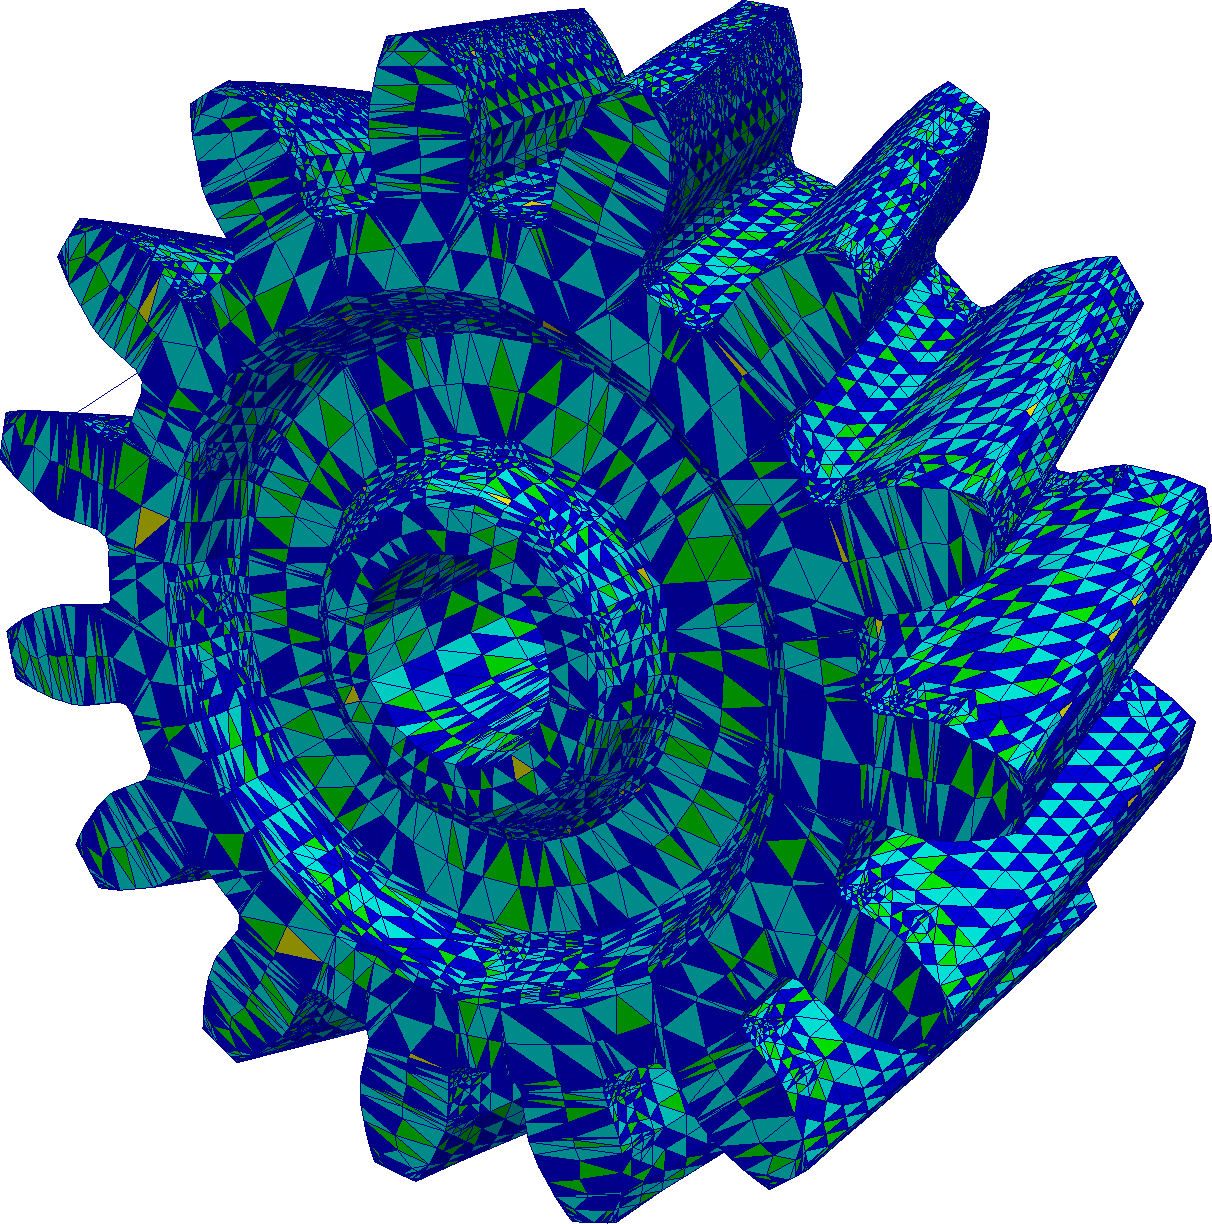
\includegraphics[width=0.5\textwidth]{chapters/logg-2/png/coloured.png}
      &
      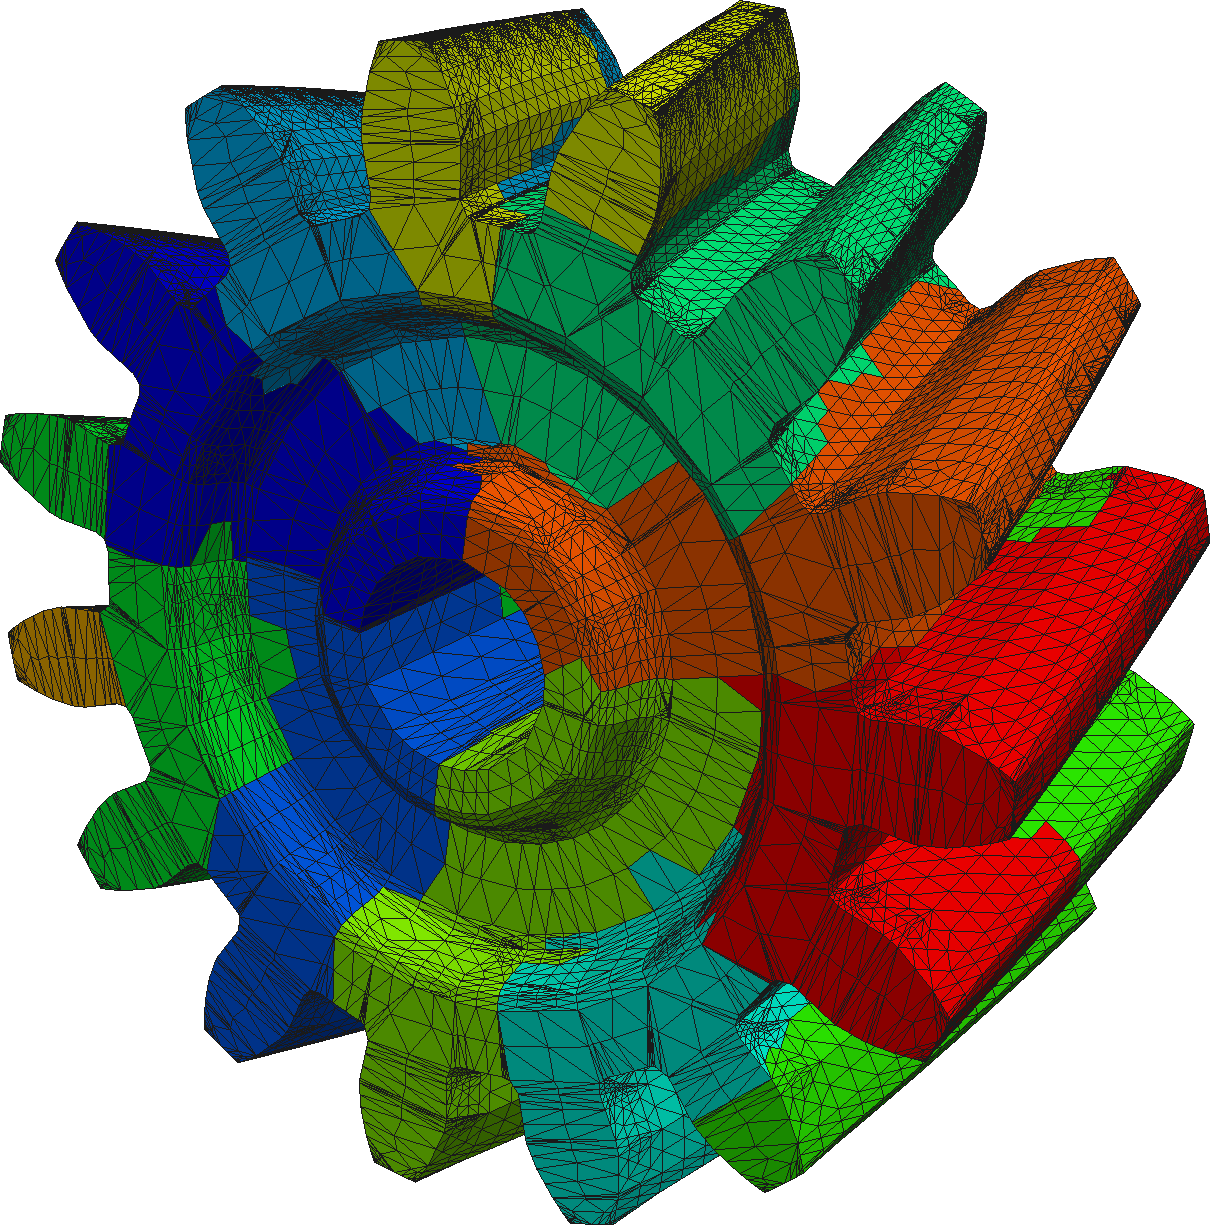
\includegraphics[width=0.5\textwidth]{chapters/logg-2/png/partition.png}
      \\[1ex] (a) & (b)
    \end{tabular}
    \caption{A mesh that is (a) colored based on facet connectivity such
     that cells that share a common facet have different colors and
     (b) partitioned into 12 parts, with each partition indicated by
     a color.}
    \label{fig:logg-2:parallel}
\end{figure}


%------------------------------------------------------------------------------
\paragraph{Shared memory parallel computing.}

Multithreaded assembly for finite element matrices and vectors on shared
memory machines is supported using OpenMP. It is activated by
setting the number of threads to use via the parameter system.
For example, the code
%%
\begin{c++}
parameters["num_threads"] = 6;
\end{c++}
%%
instructs DOLFIN to use six threads in the assembly process.  During
assembly, DOLFIN loops over the cells or cell facets in a mesh, and
computes local contributions to the global matrix or vector, which are
then added to the global matrix or vector. When using multithreaded
assembly, each thread is assigned a collection of cells or facets for
which it is responsible. This is transparent to the user.

The use of multithreading requires design care to avoid race conditions,
which occur if multiple threads attempt to write to the same memory
location at the same time.  Race conditions will typically result in
unpredictable behavior of a program. To avoid race conditions during
assembly, which would occur if two threads were to add values to a global
matrix or vector at almost the same time, DOLFIN uses a graph coloring
approach.  Before assembly, the mesh on a given process is `colored'
such that each cell is assigned a color (which in practice is an integer)
and such that no two neighboring cells have the same color. The sense
in which cells are neighbors for a given problem depends on the type
of finite element being used. In most cases, cells that share a vertex
are considered neighbors, but in other cases cells that share edges or
facets may be considered neighbors. During assembly, cells are assembled
by color. All cells of the first color are shared among the threads
and assembled, and this is followed by the next color. Since cells of
the same color are not neighbors, and therefore do not share entries in the
global matrix or vector, race conditions will not occur during assembly.
The coloring of a mesh is performed in DOLFIN using either the interface
to the Boost Graph Library or the interface to Zoltan (which is part of
the Trilinos project).  Figure~\ref{fig:logg-2:parallel}a shows a mesh
that has been colored such that no two neighboring cells (in the sense
of a shared facet) are of the same color.

Multithreaded support in third-party linear algebra libraries is limited
at the present time, but is an area of active development.  The LU solver
\citet{www:pastix}, which can be accessed via the PETSc linear algebra
backend, supports multithreaded parallelism.

%------------------------------------------------------------------------------
\paragraph{Distributed parallel computing.}

Fully distributed parallel computing is supported using the Message
Passing Interface (MPI). To perform parallel simulations, DOLFIN should
be compiled with MPI and a parallel linear algebra backend (such as PETSc
or Trilinos) enabled. To execute a parallel simulation, a DOLFIN program
should be launched using \emp{mpirun} (the name of the program to launch MPI
programs may differ on some computers). A C++ program using 16 processes
can be executed using:
%%
\begin{bash}
mpirun -n 16 ./myprogram
\end{bash}
%%
and for Python:
%%
\begin{bash}
mpirun -n 16 python myprogram.py
\end{bash}

DOLFIN supports fully distributed parallel meshes, which means that each
processor has a copy of only the portion of the mesh for which it is
responsible. This approach is scalable since no processor is required
to hold a copy of the full mesh.
An important step in a parallel simulation is the partitioning of the
mesh. DOLFIN can perform mesh partitioning in parallel using the libraries
\citet{www:parmetis} and SCOTCH \citep{www:scotch}.  The library to be
used for mesh partitioning can be specified via the parameter system,
e.g., to use SCOTCH:
%%
\begin{c++}
parameters["mesh_partitioner"] = "SCOTCH";
\end{c++}
%%
or to use ParMETIS:
%%
\begin{python}
parameters["mesh_partitioner"] = "ParMETIS"
\end{python}
%%
Figure~\ref{fig:logg-2:parallel}b shows a mesh that has been partitioned
in parallel into 12 domains. One process would take responsibility
for each domain.

If a parallel program is launched using MPI and a parallel linear
algebra backend is enabled, then linear algebra operations will be
performed in parallel. In most applications, this will be transparent
to the user.  Parallel output for postprocessing is supported through
the PVD output format, and is used in the same way as for serial
output. Each process writes an output file, and the single main output
file points to the files produced by the different processes.

%------------------------------------------------------------------------------
\subsection{Implementation and generation of the Python interface}

The DOLFIN C++ library is wrapped to Python using the Simplified
Wrapper and Interface Generator \swig \citep{Beazley2006,www:swig}
(see Chapter~\ref{chap:mardal-2} for more details). The wrapped C++
library is accessible in a Python module named \emp{cpp} residing inside the
main \emp{dolfin} module of DOLFIN. This means that the compiled
module, with all its functions and classes, can be accessed directly
by:
%%
\begin{python}
from dolfin import cpp
Function = cpp.Function
assemble = cpp.assemble
\end{python}
%%
The classes and functions in the \emp{cpp} module have the same
functionality as the corresponding classes and functions in the C++
interface. In addition to the wrapper layer automatically generated
by SWIG, the DOLFIN Python interface relies on a number of components
implemented directly in Python. Both are imported into the Python module
named \emp{dolfin}. In the following sections, the key customizations to
the DOLFIN interface that facilitate this integration are presented. The
Python interface also integrates well with the \numpy and \scipy toolkits,
which is also discussed below.

%------------------------------------------------------------------------------
\subsection{UFL integration and just-in-time compilation}

In the Python interface, the UFL form language has been integrated
with the Python wrapped DOLFIN C++ module.  When explaining the
integration, we use in this section the notation \emp{dolfin::Foo}
or \emp{dolfin::bar} to denote a C++ class or function in \dolfin. The
corresponding \swig-wrapped classes or functions will be referred to
as \emp{cpp.Foo} and \emp{cpp.bar}. A class in UFL will be referred
to as \emp{ufl.Foo} and a class in \ufc as \emp{ufc::foo} (note lower
case). The Python classes and functions in the added Python layer on
top of the wrapped C++ library, will be referred to as \emp{dolfin.Foo}
or \emp{dolfin.bar}. The prefixes of the classes and functions are
sometimes skipped for convenience. Most of the code snippets presented
in this section are pseudo code. Their purpose is to illustrate the
logic of a particular method or function. Parts of the actual code may
be intentionally excluded. A reader can examine particular classes or
functions in the code for a full understanding of the implementation.

\paragraph{Construction of function spaces}

In the Python interface, \emp{ufl.FiniteElement} and
\emp{dolfin::FunctionSpace} are integrated. The declaration of a
\emp{FunctionSpace} is similar to that of a \emp{ufl.FiniteElement},
but instead of a cell type (for example, \emp{triangle}) the
\emp{FunctionSpace} constructor takes a \emp{cpp.Mesh} (\emp{dolfin.Mesh}):
%%
\begin{python}
mesh = UnitSquare(8, 8)
V = FunctionSpace(mesh, "Lagrange", 1)
\end{python}
%%
In the Python constructor of \emp{FunctionSpace}, a
\emp{ufl.FiniteElement} is instantiated. The \emp{FiniteElement}
is passed to a just-in-time (JIT) compiler, which returns compiled
and Python-wrapped \emp{ufc} objects: a \emp{ufc::finite\_element}
and a \emp{ufc::dofmap}. These two objects, together with the mesh,
are used to instantiate a \emp{cpp.FunctionSpace}. The following pseudo
code illustrates the instantiation of a \emp{FunctionSpace} from the
Python interface:
%%
\begin{python}
class FunctionSpace(cpp.FunctionSpace):
    def __init__(self, mesh, family, degree):
        # Figure out the domain from the mesh topology
        if mesh.topology().dim() == 2:
            domain = ufl.triangle
        else:
            domain = ufl.tetrahedron

        # Create the UFL FiniteElement
        self.ufl_element = ufl.FiniteElement(family, domain, degree)

        # JIT compile and instantiate the UFC classes
        ufc_element, ufc_dofmap = jit(self.ufl_element)

        # Instantiate DOLFIN classes and finally the FunctionSpace
        dolfin_element = cpp.FiniteElement(ufc_element)
        dolfin_dofmap = cpp.DofMap(ufc_dofmap, mesh)
        cpp.FunctionSpace.__init__(self, mesh, dolfin_element, dolfin_dofmap)
\end{python}

\paragraph{Constructing arguments (trial and test functions)}

The \emp{ufl.Argument} class (the base class of \emp{ufl.TrialFunction}
and \emp{ufl.TestFunction}) is subclassed in the Python interface. Instead
of using a \emp{ufl.FiniteElement} to instantiate the classes, a DOLFIN
\emp{FunctionSpace} is used:
%%
\begin{python}
u = TrialFunction(V)
v = TestFunction(V)
\end{python}
%%
The \emp{ufl.Argument} base class is instantiated in the subclassed
constructor by extracting the \emp{ufl.FiniteElement} from the passed
\emp{FunctionSpace}, which is illustrated by the following pseudo
code:
%%
\begin{python}
class Argument(ufl.Argument):
    def __init__(self, V, index=None):
        ufl.Argument.__init__(self, V.ufl_element, index)
        self.V = V
\end{python}
%%
The \emp{TrialFunction} and \emp{TestFunction} are then defined using the
subclassed \emp{Argument} class:
%%
\begin{python}
def TrialFunction(V):
    return Argument(V, -1)

def TestFunction(V):
    return Argument(V, -2)
\end{python}

\paragraph{Coefficients, functions and expressions.}

When a UFL form is defined using a \emp{Coefficient}, a user must
associate with the form either a discrete finite element
\emp{Function} or a user-defined \emp{Expression} before the form is
assembled. In the C++ interface of DOLFIN, a user needs to explicitly
carry out this association (\emp{L.f = f}). In the Python interface of
DOLFIN, the \emp{ufl.Coefficient} class is combined with the \dolfin
\emp{Function} and \emp{Expression} classes, and the association
between the coefficient as a symbol in the form expression
(\emp{Coefficient}) and its value (\emp{Function} or \emp{Expression})
is automatic. A user can therefore assemble a form defined using
instances of these combined classes directly:
%%
\begin{python}
class Source(Expression):
    def eval(self, values, x):
        values[0] = sin(x[0])

v = TestFunction(V)
f = Source()
L = f*v*dx
b = assemble(L)
\end{python}
%%
The \emp{Function} class in the Python interface inherits from both
\emp{ufl.Coefficient} and \emp{cpp.Function}, as illustrated by the
following pseudo code:
%%
\begin{python}
class Function(ufl.Coefficient, cpp.Function):
    def __init__(self, V):
        ufl.Coefficient.__init__(self, V.ufl_element)
        cpp.Function().__init__(self, V)
\end{python}
%%
The actual constructor also includes logic to instantiate a Function
from other objects. A more elaborate logic is also included to handle
access to subfunctions.

A user-defined \emp{Expression} can be created in two different ways:
(i)~as a pure Python \emp{Expression}; or (ii)~as a JIT compiled
\emp{Expression}. A pure Python \emp{Expression} is an object instantiated
from a subclass of \emp{Expression} in Python. The \emp{Source} class
above is an example of this. Pseudo code for the constructor of the
\emp{Expression} class is similar to that for the \emp{Function} class:
%%
\begin{python}
class Expression(ufl.Coefficient, cpp.Expression):
    def __init__(self, element=None):
        if element is None:
            element = auto_select_element(self.value_shape())
        ufl.Coefficient.__init__(self, element)
        cpp.Expression(element.value_shape())
\end{python}
%%
If the \emp{ufl.FiniteElement} is not defined by the user, DOLFIN will
automatically choose an element using the \emp{auto\_select\_element}
function. The function takes the value shape of the \emp{Expression}
as argument. This has to be supplied by the user for any vector- or
tensor-valued \emp{Expression}s, by overloading the \emp{value\_shape}
method. The base class \emp{cpp.Expression} is initialized using the
value shape of the \emp{ufl.FiniteElement}.

The actual code is considerably more complex than indicated above, as
the same class, \emp{Expression}, is used to handle both JIT compiled
and pure Python \emp{Expression}s. Also note that the actual subclass
is eventually generated by a \emph{metaclass} in Python, which makes it
possible to include sanity checks for the declared subclass.

The \emp{cpp.Expression} class is wrapped by a so-called \emph{director class} in
the \swig-generated C++ layer. This means that the whole Python class is
wrapped by a C++ subclass of \emp{dolfin::Expression}. Each virtual method
of the C++ base class is implemented by the \swig-generated subclass in
C++. These methods call the Python version of the method, which the user
eventually implements by subclassing \emp{cpp.Expression} in Python.

\paragraph{Just-in-time compilation of expressions.}

The performance of a pure Python \emp{Expression} may be suboptimal
because of the callback from C++ to Python each time the \emp{Expression}
is evaluated. To circumvent this, a user can instead subclass the C++
version of \emp{Expression} using a JIT compiled \emp{Expression}. Because
the subclass is implemented in C++, it will not involve any callbacks
to Python, and can therefore be significantly faster than a pure Python
\emp{Expression}. A JIT compiled \emp{Expression} is generated by passing
a string of C++ code to the \emp{Expression} constructor:
%%
\begin{python}
e = Expression("sin(x[0])")
\end{python}
%%
The passed string is used to generate a subclass of
\emp{dolfin::Expression} in C++, where it is inlined into an overloaded
\emp{eval} method. The final code is JIT compiled and wrapped to Python
using \instant (see Chapter~\ref{chap:wilbers}). The generated Python
class is then imported into Python. The class is not yet instantiated,
as the final JIT compiled \emp{Expression} also needs to inherit from
\emp{ufl.Coefficient}. To accomplish this, we dynamically create a class
which inherits from both the generated class and \emp{ufl.Coefficient}.

Classes in Python can be created during run-time by using the
\emp{type} function. The logic of creating a class and returning an
instance of that class is handled in the \emp{\_\_new\_\_} method of
\emp{dolfin.Expression}, as illustrated by the following pseudo code:
%%
\begin{python}
class Expression(object):
    def __new__(cls, cppcode=None):
        if cls.__name__ != "Expression":
            return object.__new__(cls)
        cpp_base = compile_expressions(cppcode)
        def __init__(self, cppcode):
            ...
        generated_class = type("CompiledExpression",
                               (Expression, ufl.Coefficient, cpp_base),
                               {"__init__": __init__})
        return generated_class()
\end{python}
%%
The \emp{\_\_new\_\_} method is called when a JIT compiled
\emp{Expression} is instantiated. However, it will also be called
when a pure Python subclass of \emp{Expression} is instantiated during
initialization of the base-class. We handle the two different cases by
checking the name of the instantiated class. If the name of the class is
not \emp{"Expression"} then the call originates from the instantiation
of a subclass of \emp{Expression}. When a pure Python \emp{Expression}
is instantiated, like the \emp{Source} instance in the code example
above, the \emp{\_\_new\_\_} method of \emp{object} is called and the
instantiated object is returned.  In the other case, when a JIT compiled
\emp{Expression} is instantiated, we need to generate the JIT compiled
base class from the passed Python string, as explained above. This
is done by calling the function \emp{compile\_expressions}. Before
\emp{type} is called to generate the final class, an \emp{\_\_init\_\_}
method for the class is defined. This method initiates the new object
by automatically selecting the element type and setting dimensions
for the created \emp{Expression}. This procedure is similar to what is
done for the Python derived \emp{Expression} class, see above. Finally,
we construct the new class which inherits the JIT compiled class and
\emp{ufl.Coefficient} by calling \emp{type}.

The \emp{type} function takes three arguments: the name of the class
(\emp{"CompiledExpression"}), the bases of the class (\emp{Expression,
  ufl.Coefficient, cpp\_base}), and a \emp{dict} defining the
interface (methods and attributes) of the class. The only new method or
attribute we provide to the generated class is the \emp{\_\_init\_\_}
method. After the class is generated, we instantiate it and the object
is returned to the user.


\paragraph{Assembly of UFL forms.}

The \emp{assemble} function in the Python interface of DOLFIN enables
a user to directly assemble a declared UFL form:
%%
\begin{python}
mesh = UnitSquare(8, 8)
V = FunctionSpace("CG", mesh, 1)
u = TrialFunction(V)
v = TestFunction(V)
c = Expression("sin(x[0])")
a = c*dot(grad(u), grad(v))*dx
A = assemble(a)
\end{python}
%%
The \emp{assemble} function is a thin wrapper layer around the wrapped
\emp{cpp.assemble} function. The following pseudo code illustrates what
happens in this layer:
%%
\begin{python}
def assemble(form, tensor=None, mesh=None):
    dolfin_form = Form(form)
    if tensor is None:
        tensor = create_tensor(dolfin_form.rank())
    if mesh is not None:
        dolfin_form.set_mesh(mesh)
    cpp.assemble(dolfin_form, tensor)
    return tensor
\end{python}
%%
Here, \emp{form} is a \emp{ufl.Form}, which is used to generate a
\emp{dolfin.Form}, as explained below. In addition to the \emp{form}
argument, a user can choose to provide a tensor and/or a mesh. If a
tensor is not provided, one will automatically be generated by the
\emp{create\_tensor} function. The optional mesh is needed if the form
does not contain any \emp{Argument}s, or \emp{Function}s; for example
when a functional containing only \emp{Expression}s is assembled. Note
that the length of the above signature has been shortened. Other
arguments to the \emp{assemble} function exist but are skipped here
for clarity.

The following pseudo code demonstrates what happens in the constructor
of \emp{dolfin.Form}, where the base class \emp{cpp.Form} is initialized
from a \emp{ufl.Form}:
%%
\begin{python}
class Form(cpp.Form):
    def __init__(self, form):
        compiled_form, form_data = jit(form)
        function_spaces = extract_function_spaces(form_data)
        coefficients = extract_coefficients(form_data)
        cpp.Form.__init__(self, compiled_form, function_spaces, coefficients)
\end{python}
%%
The \emp{form} is first passed to the \emp{dolfin.jit} function,
which calls the registered form compiler to generate code and JIT
compile it. There are presently two form compilers that can be
chosen: \emp{"ffc"} and \emp{"sfc"} (see Chapters~\ref{chap:logg-1}
and~\ref{chap:alnes-3}). Each one of these form compilers defines its
own \emp{jit} function, which eventually will receive the call. The form
compiler can be chosen by setting:
%%
\begin{python}
parameters["form_compiler"]["name"] = "sfc"
\end{python}
%%
The default form compiler is \emp{"ffc"}. The \emp{jit} function
of the form compiler returns the JIT compiled \emp{ufc::form}
together with a \emp{ufl.FormData} object. The latter is a data
structure containing meta data for the \emp{ufl.form}, which is used
to extract the function spaces and coefficients that are needed to
instantiate a \emp{cpp.Form}. The extraction of this data is handled by
the \emp{extract\_function\_spaces} and the \emp{extract\_coefficients}
functions.

%------------------------------------------------------------------------------
\subsection{\numpy and \scipy integration}

The values of the \emp{Matrix} and \emp{Vector} classes in the Python
interface of DOLFIN can be viewed as \numpy arrays. This is done by
calling the \emp{array} method of the vector or matrix:
%%
\begin{python}
A  = assemble(a)
AA = A.array()
\end{python}
%%
Here, \emp{A} is a matrix assembled from the form \emp{a}. The \numpy
array \emp{AA} is a dense structure and all values are copied from the
original data. The \emp{array} function can be called on a distributed
matrix or vector, in which case it will return the locally stored
values.

% Removed comment about calling array on a distributed matrix. What
% it does is that it returns the submatrix for the rows stored on the
% local process by calling MatGetRow for those rows.


\paragraph{Direct access to linear algebra data.}

Direct access to the underlying data is possible for the \emp{uBLAS}
and \emp{MTL4} linear algebra backends. A \numpy array view into the
data will be returned by the method \emp{data}:
%%
\begin{python}
parameters["linear_algebra_backend"] = "uBLAS"
b  = assemble(L)
bb = b.data()
\end{python}
%%
Here, \emp{b} is a \emp{uBLAS} vector and \emp{bb} is a \numpy view
into the data of \emp{b}. Any changes to \emp{bb} will directly affect
\emp{b}. A similar method exists for matrices:
%%
\begin{python}
parameters["linear_algebra_backend"] = "MTL4"
A = assemble(a)
rows, columns, values = A.data()
\end{python}
%%
The data is returned in a compressed row storage format as the three
\numpy arrays \emp{rows}, \emp{columns}, and \emp{values}. These are also
views of the data that represent \emp{A}. Any changes in \emp{values}
will directly result in a corresponding change in~\emp{A}.

\paragraph{Sparse matrix and SciPy integration.}

The \emp{rows}, \emp{columns}, and \emp{values} data structures can
be used to instantiate a \emp{csr\_matrix} from the \emp{scipy.sparse}
module \citep{JonesOliphantPetersonEtAl2009}:
%%
\begin{python}
from scipy.sparse import csr_matrix
rows, columns, values = A.data()
csr = csr_matrix(values, rows, columns)
\end{python}
%%
The \emp{csr\_matrix} can then be used with other Python modules
that support sparse matrices, such as the \emp{scipy.sparse}
module and \emp{pyamg}, which is an algebraic multigrid solver
\citep{BellOlsonSchroder2009}.

\paragraph{Slicing vectors.}

\numpy provides a convenient slicing interface for \numpy arrays. The
Python interface of DOLFIN also provides such an interface for vectors
(see Chapter~\ref{chap:mardal-2} for details of the implementation). A
slice can be used to access and set data in a vector:
%%
\begin{python}
# Create copy of vector
b_copy = b[:]

# Slice assignment (c can be a scalar, a DOLFIN vector or a NumPy array)
b[:] = c

# Set negative values to zero
b[b < 0] = 0

# Extract every second value
b2 = b[::2]
\end{python}
%%
A difference between a \numpy slice and a slice of a DOLFIN vector is
that a slice of a \numpy array provides a view into the original array,
whereas in DOLFIN we provide a copy. A list/tuple of integers or a \numpy
array can also be used to both access and set data in a vector:
%%
\begin{python}
b1 = b[(0, 4, 7, 10)]
b2 = b[array((0, 4, 7, 10))]
\end{python}

%------------------------------------------------------------------------------
%------------------------------------------------------------------------------
\section{Historical notes}

The first public version of DOLFIN, version~0.2.0, was released in
2002. At that time, DOLFIN was a self-contained C++ library with
minimal external dependencies. All functionality was then implemented
as part of DOLFIN itself, including linear algebra and finite element
form evaluation. Although only piecewise linear elements were
supported, DOLFIN provided rudimentary automated finite element
assembly of variational forms. The form language was implemented by
C++ operator overloading. For an overview of the development of the
FEniCS form language and an example of the early form language
implemented in DOLFIN, see Chapter~\ref{chap:logg-1}.

Later, parts of the functionality of DOLFIN have been moved to either
external libraries or other FEniCS components. In 2003, the FEniCS
project was born and shortly after, with the release of version~0.5.0 in
2004, the form evaluation system in DOLFIN was replaced by an automated
code generation system based on FFC and FIAT. In the following year,
the linear algebra was replaced by wrappers for PETSc data structures
and solvers. At this time, the DOLFIN Python interface (PyDOLFIN) was
introduced. Since then, the Python interface has developed from a simple
auto-generated wrapper layer for the DOLFIN C++ functionality to a mature
problem-solving environment with support for just-in-time compilation of
variational forms and integration with external Python modules like NumPy.

In 2006, the DOLFIN mesh data structures were simplified and
reimplemented to improve efficiency and expand functionality. The new
data structures were based on a light-weight object-oriented layer on
top of an underlying data storage by plain contiguous C/C++ arrays and
improved the efficiency by orders of magnitude over the old
implementation, which was based on a fully object-oriented
implementation with local storage of all mesh entities like cells and
vertices. The first release of DOLFIN with the new mesh library was
version~0.6.2.

In 2007, the UFC interface was introduced and the FFC form language was
integrated with the DOLFIN Python interface. Just-in-time compilation
was also introduced. The following year, the linear algebra interfaces
of DOLFIN were redesigned to allow flexible handling of multiple linear
algebra backends. In 2009, a major milestone was reached when parallel
computing was introduced in DOLFIN.

Over the years, DOLFIN has undergone a large number of changes to its
design, interface and implementation. However, since the release of
DOLFIN 0.9.0, which introduced a redesign of the DOLFIN function classes
based on the new function space abstraction, only minor changes have been
made to the interface. Since the release of version~0.9.0, most work has
gone into refining the interface, implementing missing functionality,
fixing bugs and improving documentation, in anticipation of the
first stable release of DOLFIN, version 1.0.

%%% Local Variables:
%%% mode: latex
%%% TeX-master: "../../book"
%%% End:
